%\documentclass[handout,xcolor=pdftex,dvipsnames,table,mathserif]{beamer}
\documentclass[xcolor=pdftex,dvipsnames,table]{beamer}
\usepackage{subfigure}
\usepackage{amsbsy}
\usepackage{tikz}
\usetikzlibrary{arrows}
\usepackage{amsmath,graphicx,dsfont,color}
\usepackage{amsfonts}
\usepackage{amssymb}
\usepackage{array}

\bibliographystyle{apalike}

\setbeamertemplate{bibliography item}{\insertbiblabel}
\setbeamertemplate{bibliography entry title}{}
\setbeamertemplate{bibliography entry location}{}
\setbeamertemplate{bibliography entry note}{}

%Definitiona

\newcommand{\x}{\mathbf{x}}
\newcommand{\X}{\mathbf{X}}
\newcommand{\W}{\mathbf{W}} %Weight
\newcommand{\bais}{\mathbf{b}}%Bais
\newcommand{\act}{\texttt{g}}%Activation
\newcommand{\loss}{L}
\newcommand{\pdata}{\hat{p}_{\texttt{data}}}
\newcommand{\nsize}{n}
\newcommand{\param}{\boldsymbol{\theta}}
\newcommand{\featmap}{\boldsymbol{\phi}}
\newcommand{\EV}{\mathbb{E}}









\title{Deep Learning for Image Analysis - \\
	   Learning from fewer annotations}
\author{Thomas Walter, PhD}
\date{Centre for Computational Biology (CBIO) \\
	  MINES Paris-Tech, PSL Research University \\
	  Institut Curie, PSL Research University \\
	  INSERM U900}


%To include LOGO?
%\logo{\includegraphics[width=.1\columnwidth]{MinesLogo}}
\useinnertheme{rounded}
\usecolortheme{rose}
\usepackage{mathtools}
\usepackage[absolute,overlay]{textpos}
\usepackage{newtxmath}

\usepackage{xcolor}
\definecolor{lightblue}{RGB}{0,200,255}


\setbeamertemplate{footline}[frame number]{}
\setbeamertemplate{navigation symbols}{}
\setbeamertemplate{section in toc}[square]
\setbeamertemplate{items}[square]

%% For image credits on image bottom right
\usepackage[absolute,overlay]{textpos}
\setbeamercolor{framesource}{fg=gray}
\setbeamerfont{framesource}{size=\tiny}
\newcommand{\source}[1]{\begin{textblock*}{4cm}(8.7cm,8.6cm)
    \begin{beamercolorbox}[ht=0.5cm,right]{framesource}
      \usebeamerfont{framesource}\usebeamercolor[fg]{framesource} Credits: {#1}
    \end{beamercolorbox}
\end{textblock*}}


\begin{document}

\begin{frame}
\titlepage
\end{frame}

\begin{frame}{Overview}
\tableofcontents
\end{frame}

%%%%%%%%%%%%%%%%%%%%%%%%%%%%%%%%%%%%%%%%%%%%%%%%%%%%%%%%%%%%%%%%%%%%%%%%%
%%%%%%%%%%%%%%%%%%%%%%%%%%%%%%%%%%%%%%%%%%%%%%%%%%%%%%%%%%%%%%%%%%%%%%%%%
\section{Motivation}
\frame{\frametitle{Overview}\tableofcontents[currentsection]}

\begin{frame}{Deep Learning: there is just one catch ... }
\begin{itemize}
	\item Deep Learning is today the most powerful method for image classification, segmentation and object detecction. 
   \item Deep Learning can achieve or even go beyond human performance for these tasks. 
   \item There is a snag: deep learning relies on massive annotation.
   \item Example: ImageNet contains $1.4$ million annotated images \cite{ImageNet:2015}. 
\end{itemize}
%\vspace{-.5cm}
\end{frame}

\begin{frame}{Deep Learning: there is just one catch ... }
\begin{itemize}
\item Manual image annotation is annoying.
\item Manual image annotation is expensive.
\item We need to address the need for massive image data sets, either by avoiding massive annotation or by making annotation cheap.
\end{itemize}
%\vspace{-.5cm}
\end{frame}

%%%%%%%%%%%%%%%%%%%%%%%%%%%%%%%%%%%%%%%%%%%%%%%%%%%%%%%%%%%%%%%%%%%%%%%%%
%%%%%%%%%%%%%%%%%%%%%%%%%%%%%%%%%%%%%%%%%%%%%%%%%%%%%%%%%%%%%%%%%%%%%%%%%
\section{Strategies}

\begin{frame}{Two main strategies to overcome massive image annotation}
\begin{enumerate}
   \item Use cheap annotations. 
   \item Use different annotations. 
\end{enumerate}
\vspace{2cm}
Please note:
\begin{itemize}
   \item We always need to consider what exactly we aim at predicting (e.g. the value of a pixel or the class of an image)
   \item For instance, in segmentation, annotations are expensive at the image level, but not at the pixel level: a single stroke annotates hundreds of pixels. 
\end{itemize}
\end{frame}

\begin{frame}{Image segmentation: cheap annotations?}
\begin{figure}[htb]
   \centering
   \includegraphics[width=0.7\textwidth]{../graphics/segmentation.pdf}
   \caption{Segmentation is tedious, but provides rapidly many samples.}
\end{figure}
\begin{itemize}
   \item Providing pixel-level annotations is extremely tedious.
   \item But as we are classifying pixels, we can rapidly provide hundreds of thousands of samples. 
   \item In practice however, we need to \textbf{cover the variability} to be expected at prediction time. 
   \item For this reason, we still need a reasonable amount of images (depending on the variability). 
\end{itemize}
%\vspace{-.5cm}
\end{frame}

\begin{frame}{Massive image annotation by crowd sourcing}
\begin{figure}[htb]
   \centering
   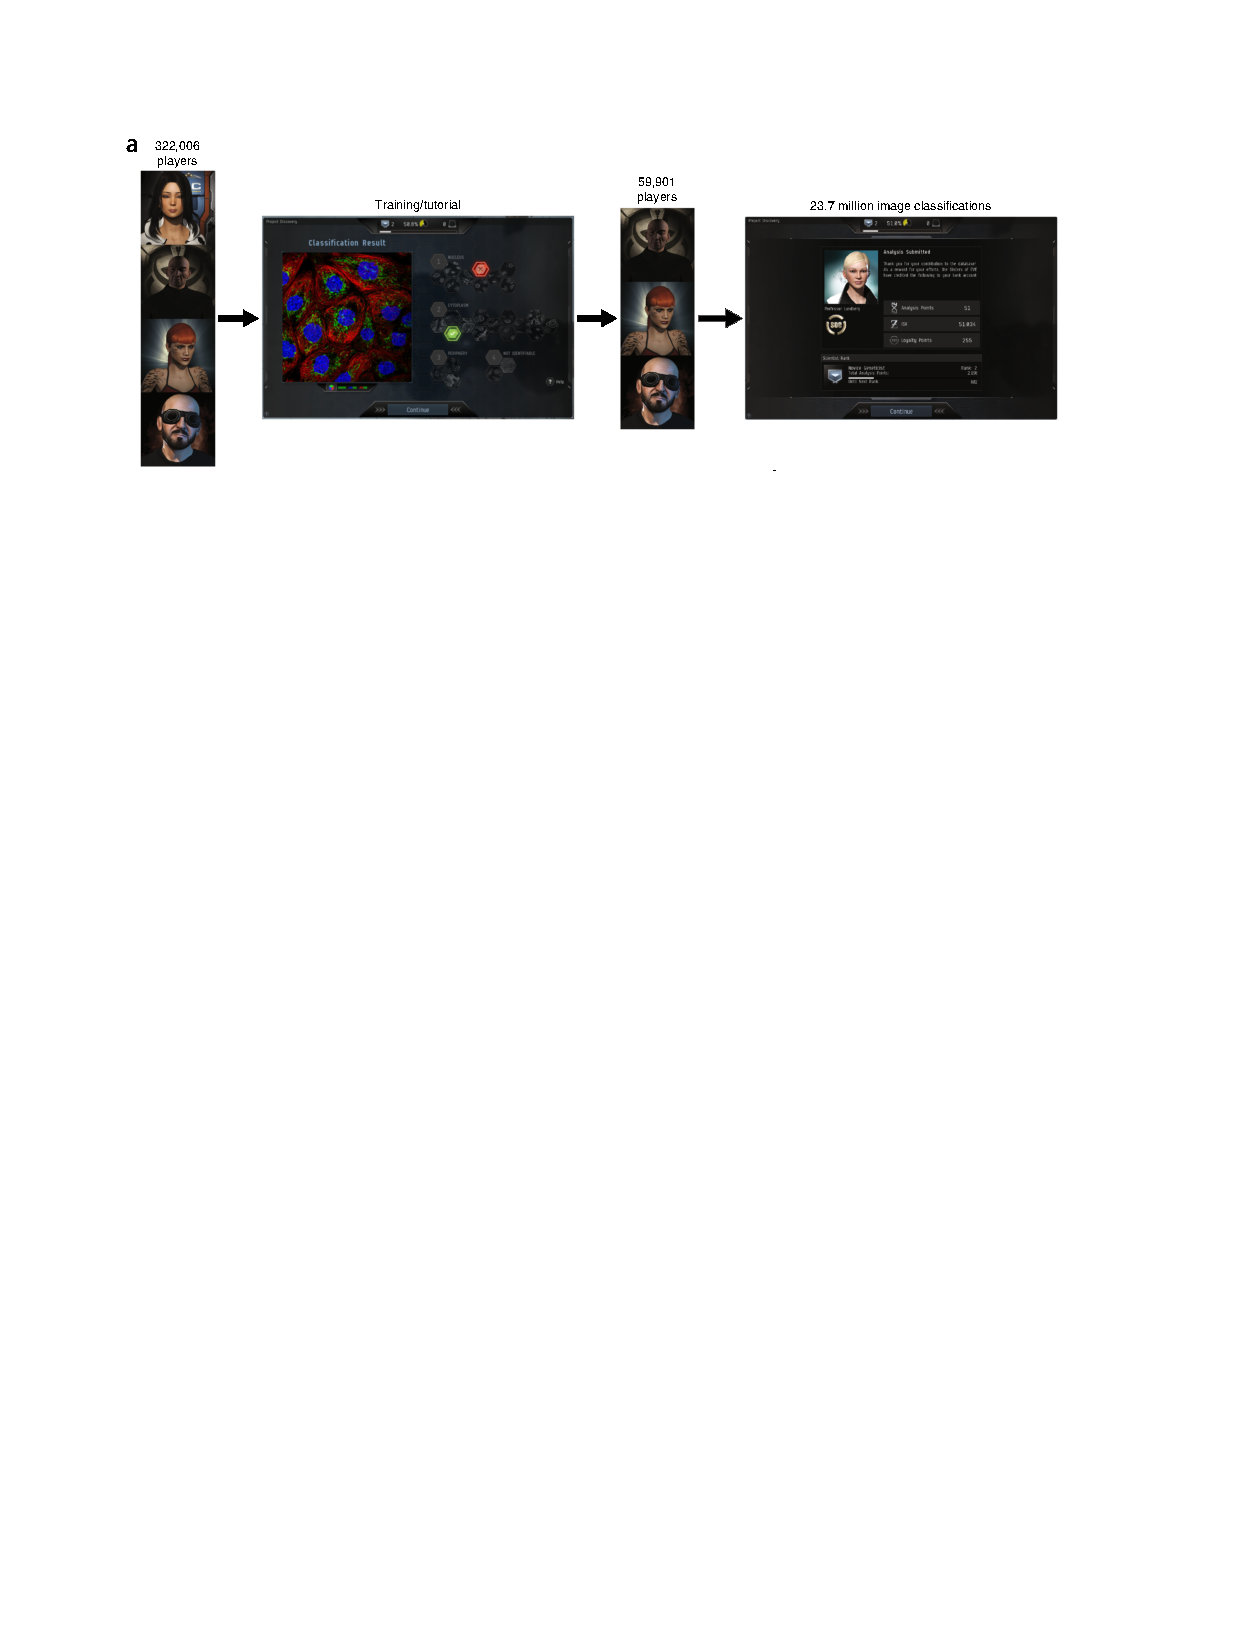
\includegraphics[width=0.85\textwidth]{../graphics/gamification.pdf}
   \caption{Gamification for the annotation of protein localization patterns: the actual annotation task is "disguised" as a computer game. Image taken from \cite{Sullivan2018a}}
\end{figure}
\begin{itemize}
   \item Crowd sourcing: generate massive annotated data sets by recruiting more people to do the annotations.
   \item This requires the implication of untrained experts (citizen science). 
   \item Several strategies to reach many people, e.g. gamification. 
\end{itemize}
%\vspace{-.5cm}
\end{frame}

\begin{frame}{Massive annotation by leveraging routinely acquired data}
\begin{figure}[htb]
   \centering
   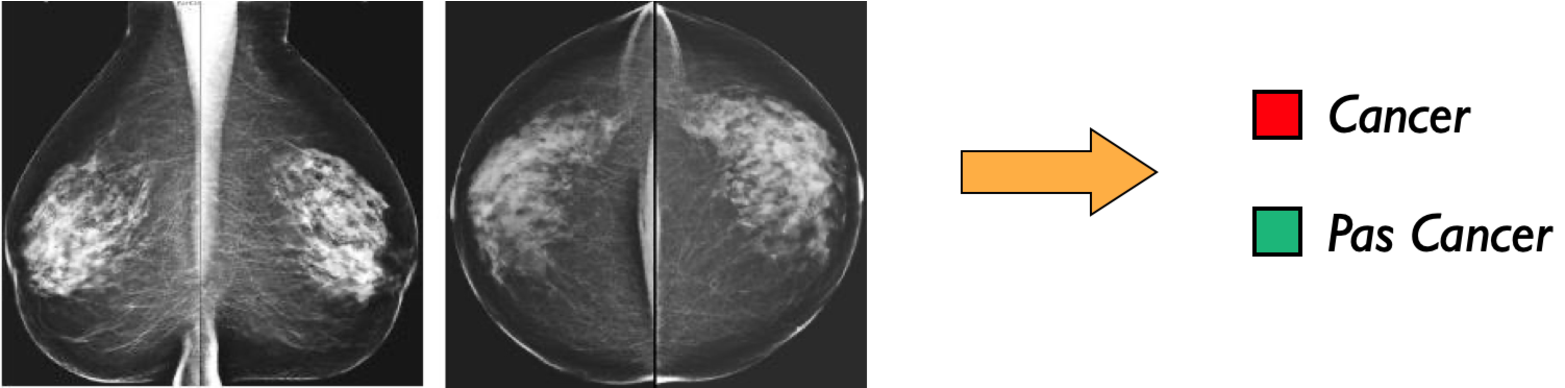
\includegraphics[width=0.7\textwidth]{../graphics/radiology.pdf}
   \caption{Radiology: mammographies are acquired routinely by physicians.}
\end{figure}
\begin{itemize}
   \item In many fields, image data is routinely acquired (e.g. medical examinations). 
   \item Origins of the image labels:
   \begin{itemize}
      \item Routine annotation by a medical doctor.
      \item Future evolution of the disease.
   \end{itemize}
   \item Problem: we are limited in the tasks, i.e. in the variables that we can predict. 
\end{itemize}
%\vspace{-.5cm}
\end{frame}

\begin{frame}{Massive image annotation by experimental design}
\begin{figure}[htb]
   \centering
   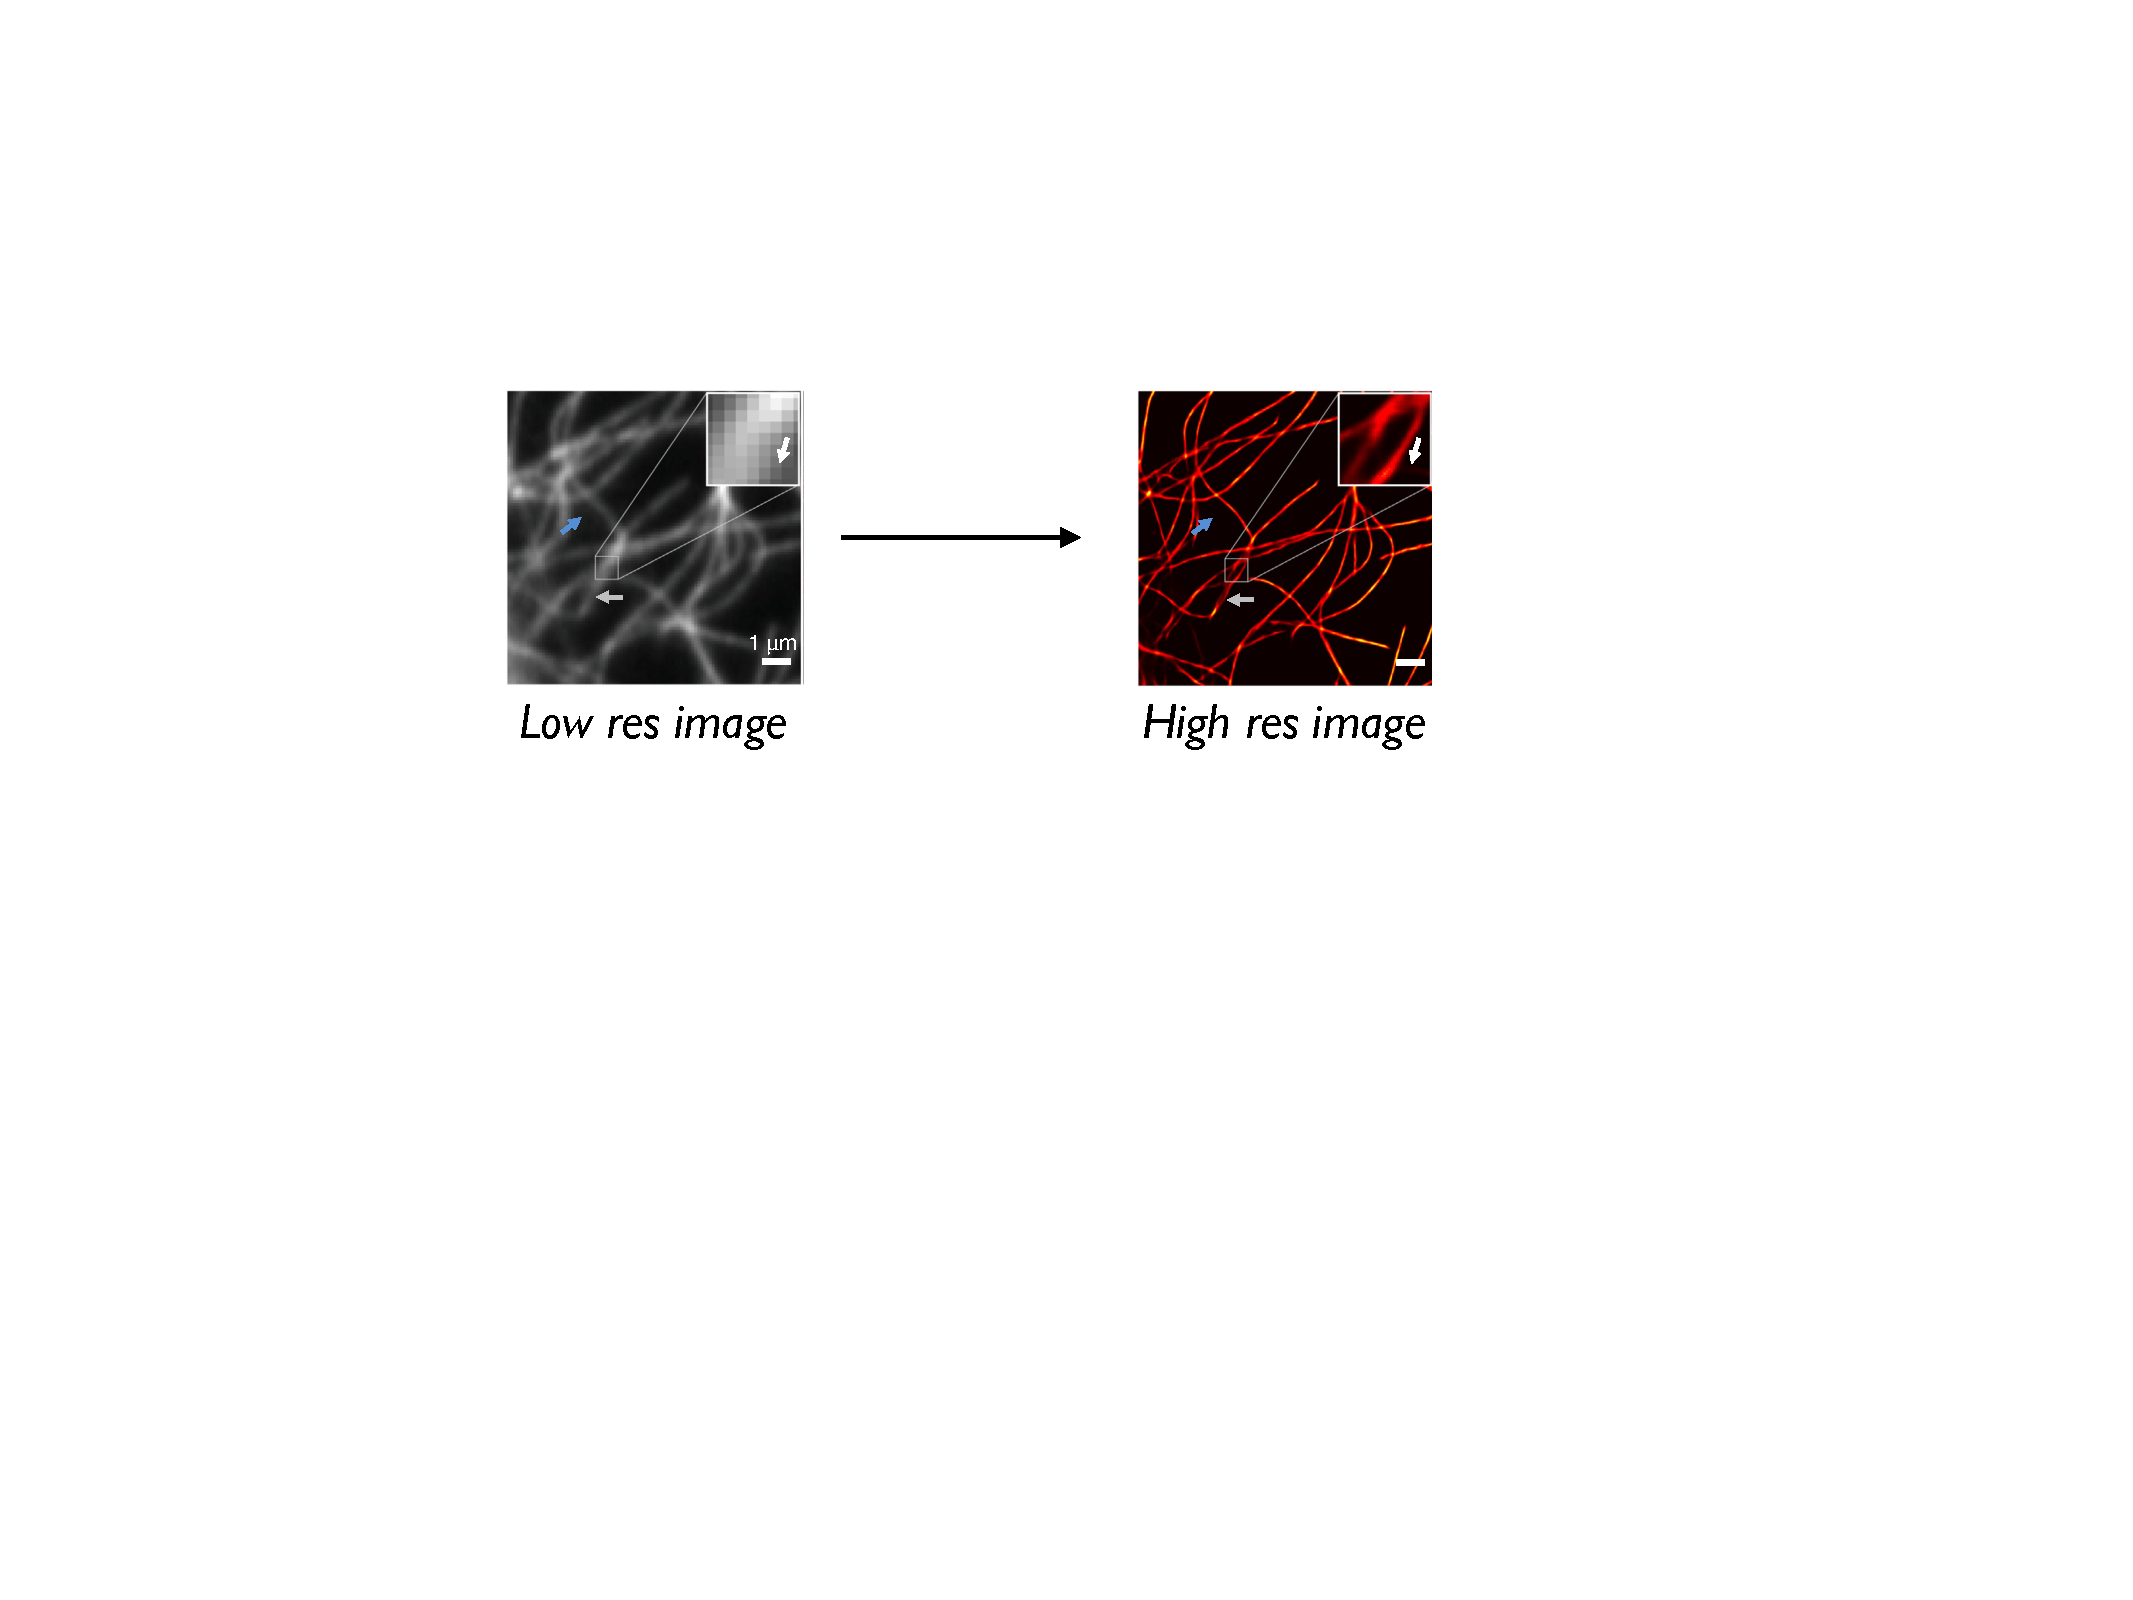
\includegraphics[width=0.7\textwidth]{../graphics/super_resolution.pdf}
   \caption{A high resolution image can be predicted from a low resolution image. Image adapted from \cite{Ouyang2018}}
\end{figure}
\begin{itemize}
   \item In image restoration, we aim at predicting a high quality image from a lower quality image. 
   \item Here, the ground-truth is entirely generated by the experimental setup (pairs of images are acquired). 
\end{itemize}
%\vspace{-.5cm}
\end{frame}

\begin{frame}{Massive image annotation by experimental design}
\begin{figure}[htb]
   \centering
   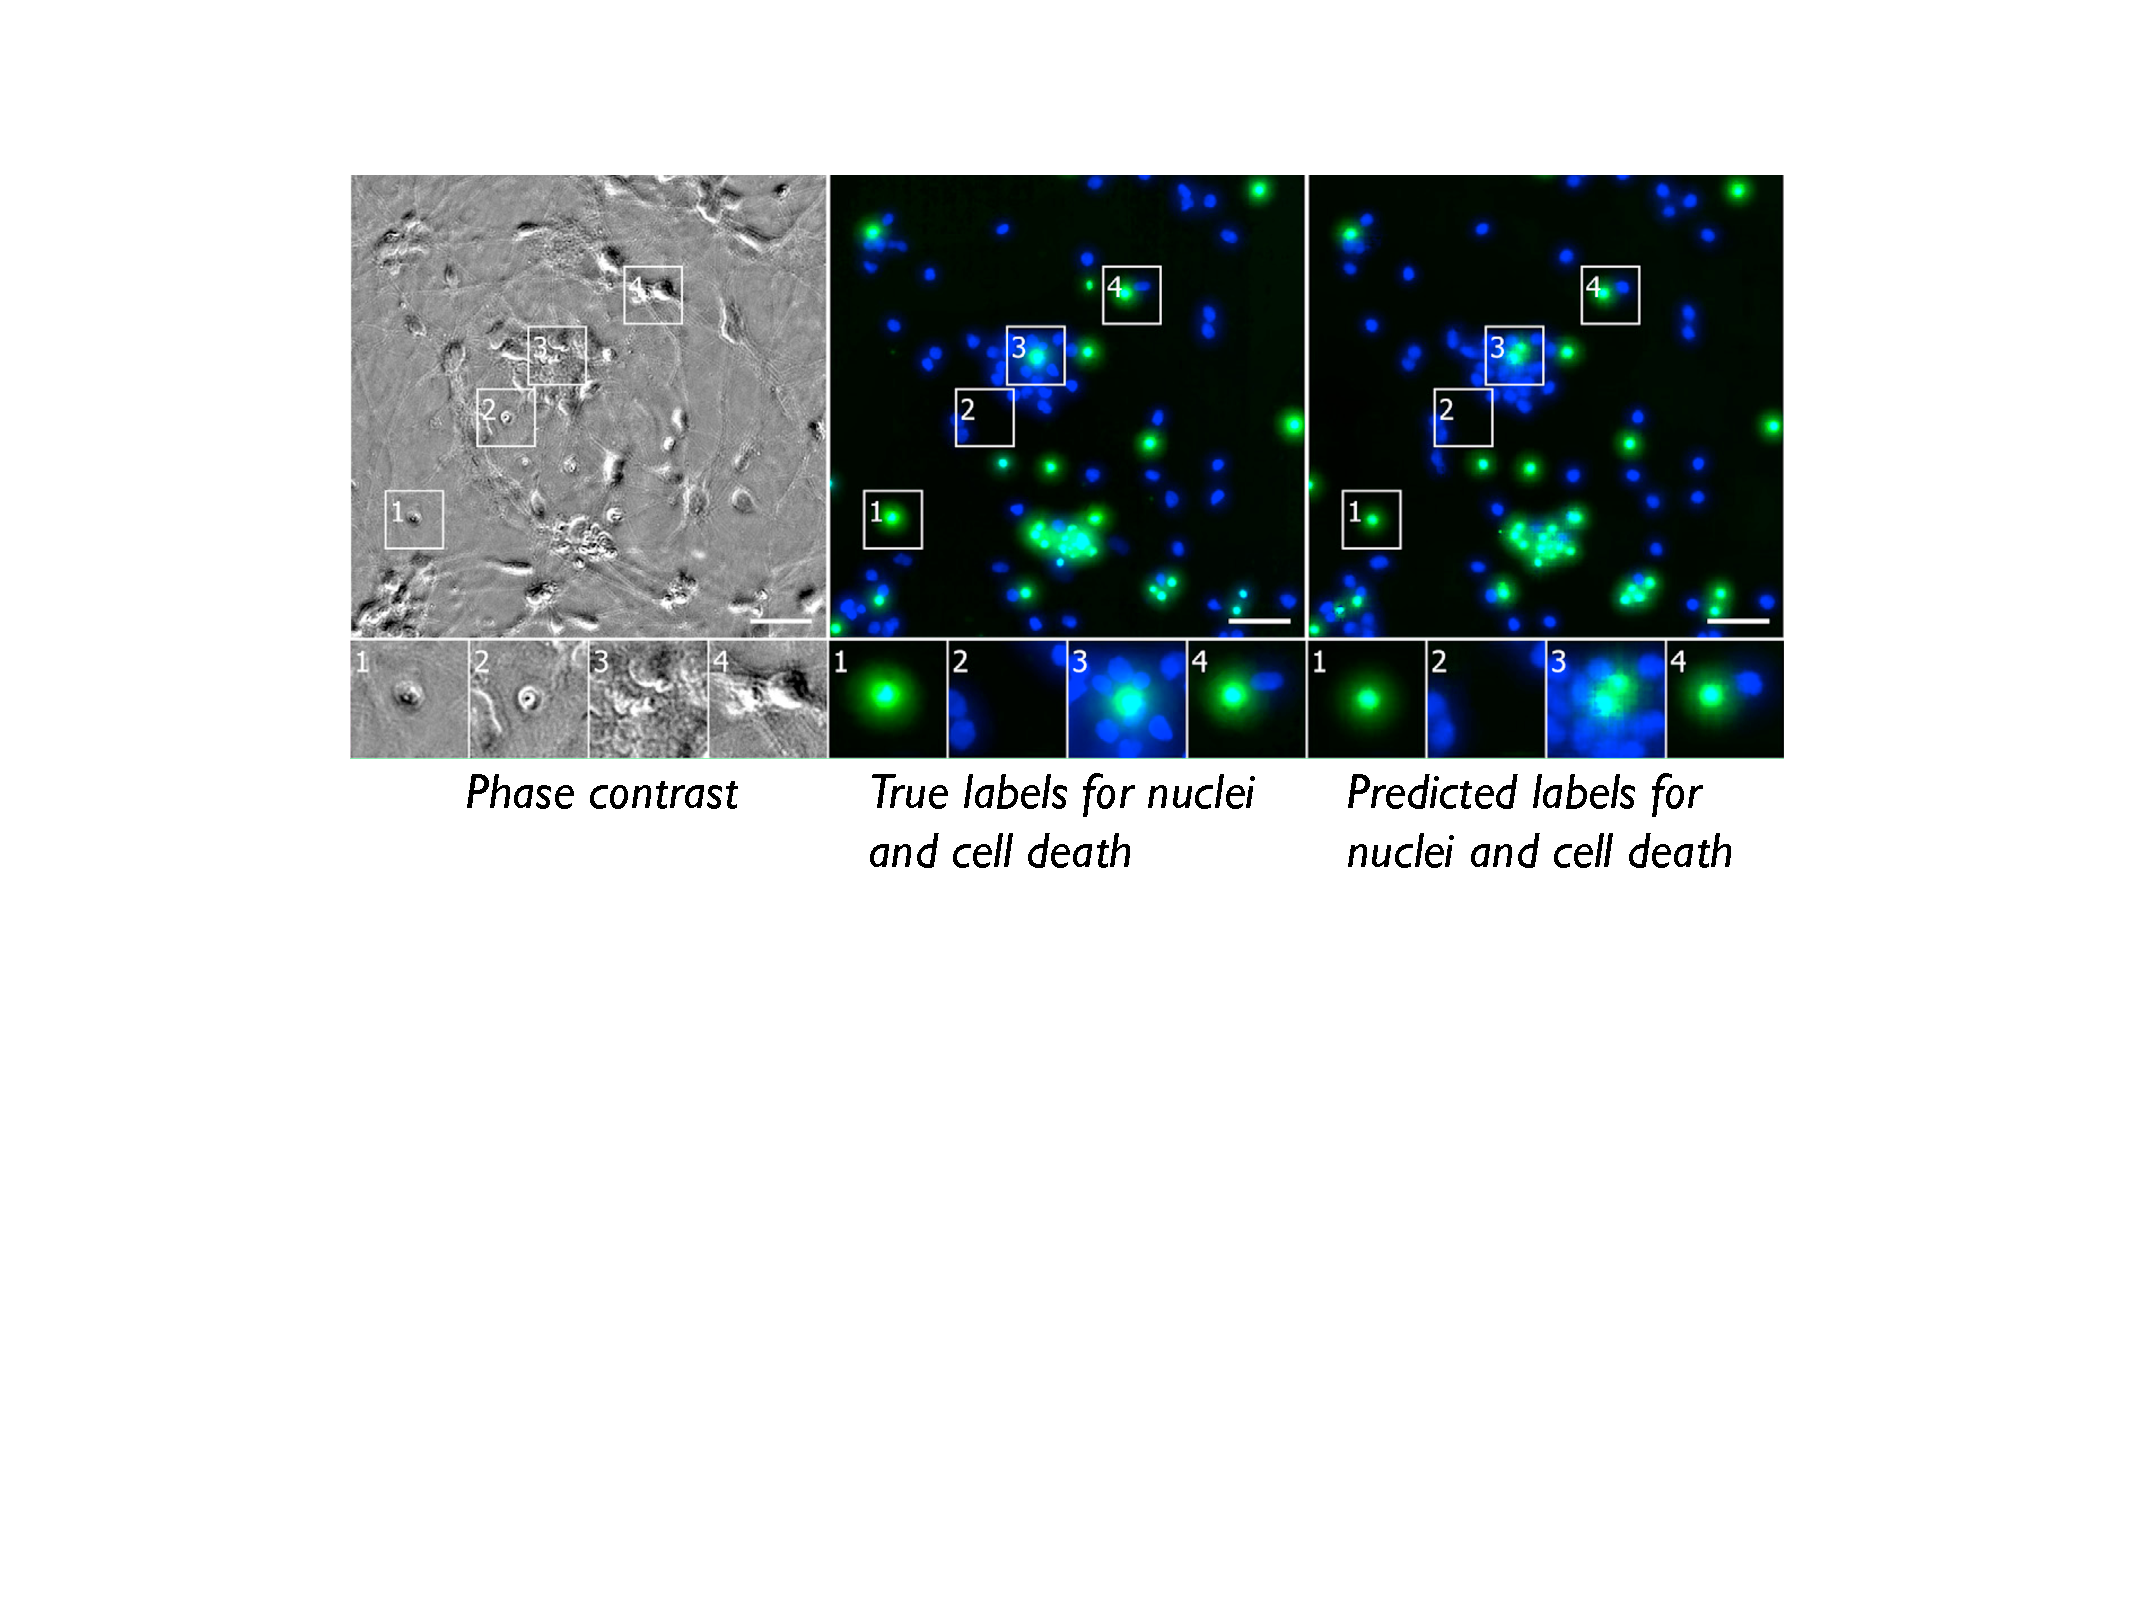
\includegraphics[width=0.7\textwidth]{../graphics/in_silico_labeling.pdf}
   \caption{Image taken with a different modality can be predicted. Here, we show an example for a fluorescent microscopy image predicted from a phase contrast microscopy image. Image adapted from \cite{Christiansen2018}}
\end{figure}
\begin{itemize}
   \item We can also predict images taken with different modalities. 
   \item This is interesting if one technique is more expensive or more invasive.
   \item Similarly, we can also use different experimental techniques to generate ground truth experimentally \cite{Boyd2020}. 
\end{itemize}
%\vspace{-.5cm}
\end{frame}


\begin{frame}{Learning from simulated data}
\begin{figure}[htb]
   \centering
   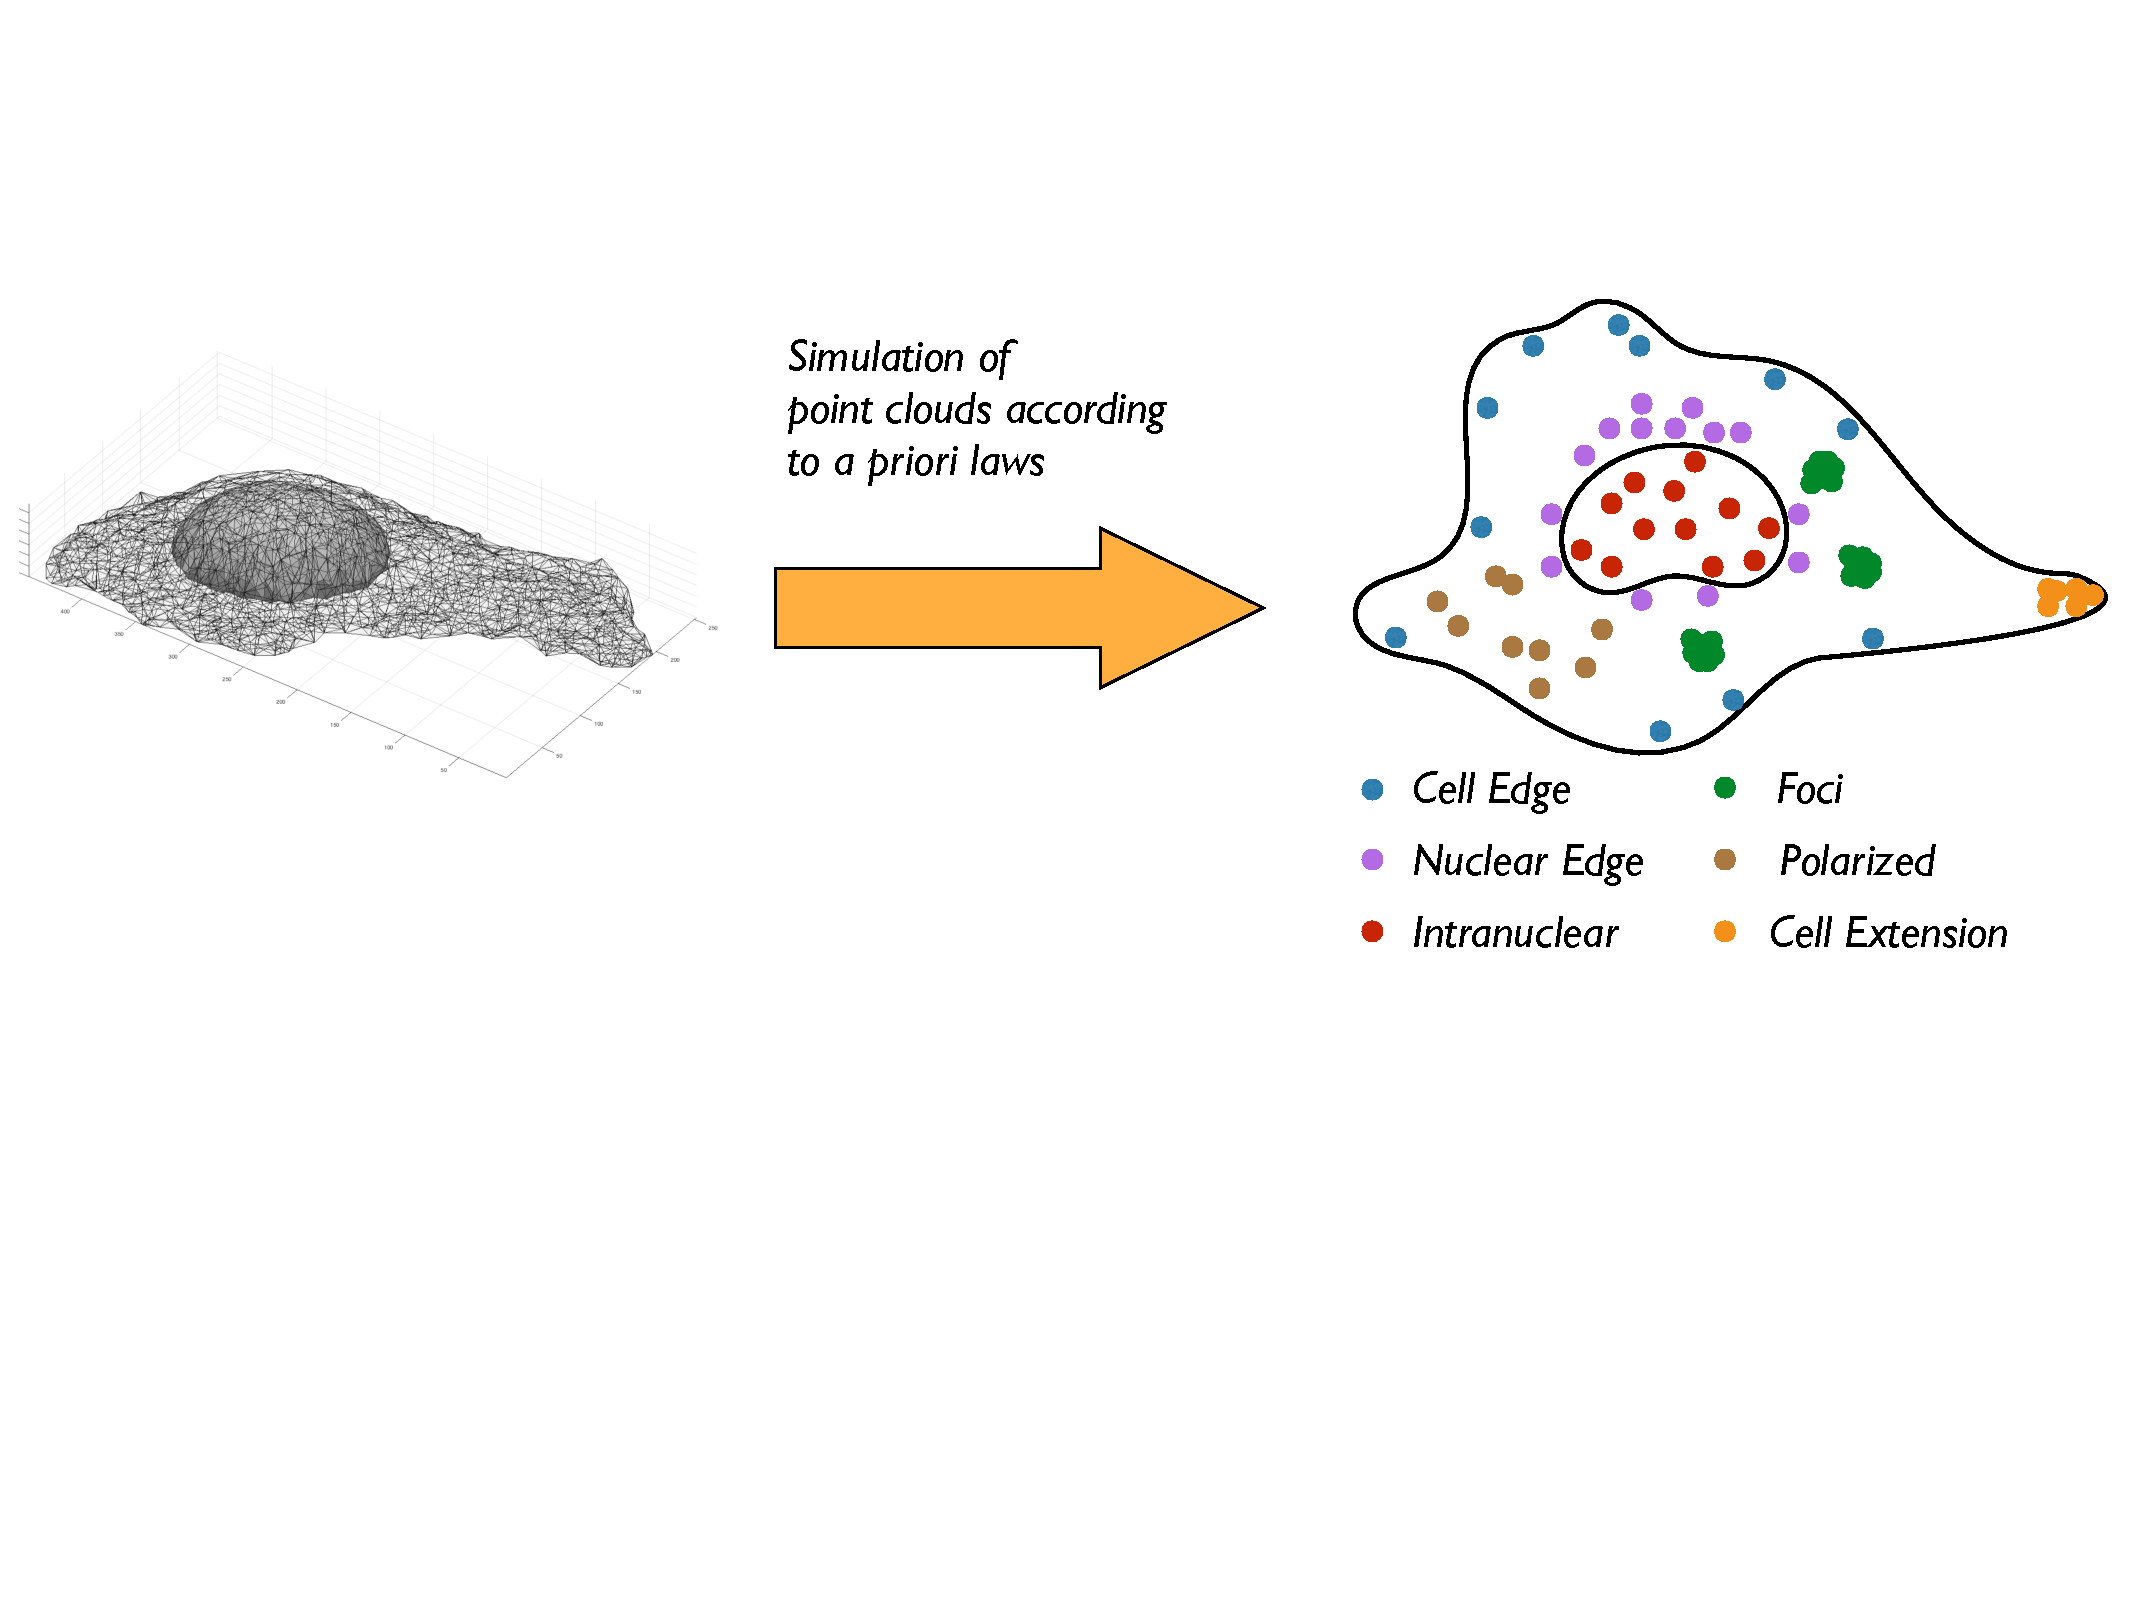
\includegraphics[width=0.95\textwidth]{../graphics/data_simulation.pdf}
   \caption{Simulated RNA localization in cells}
\end{figure}
\begin{itemize}
   \item Simulation of large amounts of data with known ground truth. 
   \item Train networks on simulated data.
   \item Problem: the data distributions between simulated and real data usually differ. 
\end{itemize}
%\vspace{-.5cm}
\end{frame}


\begin{frame}{Learning from other datasets / other tasks}
\begin{figure}[htb]
   \centering
   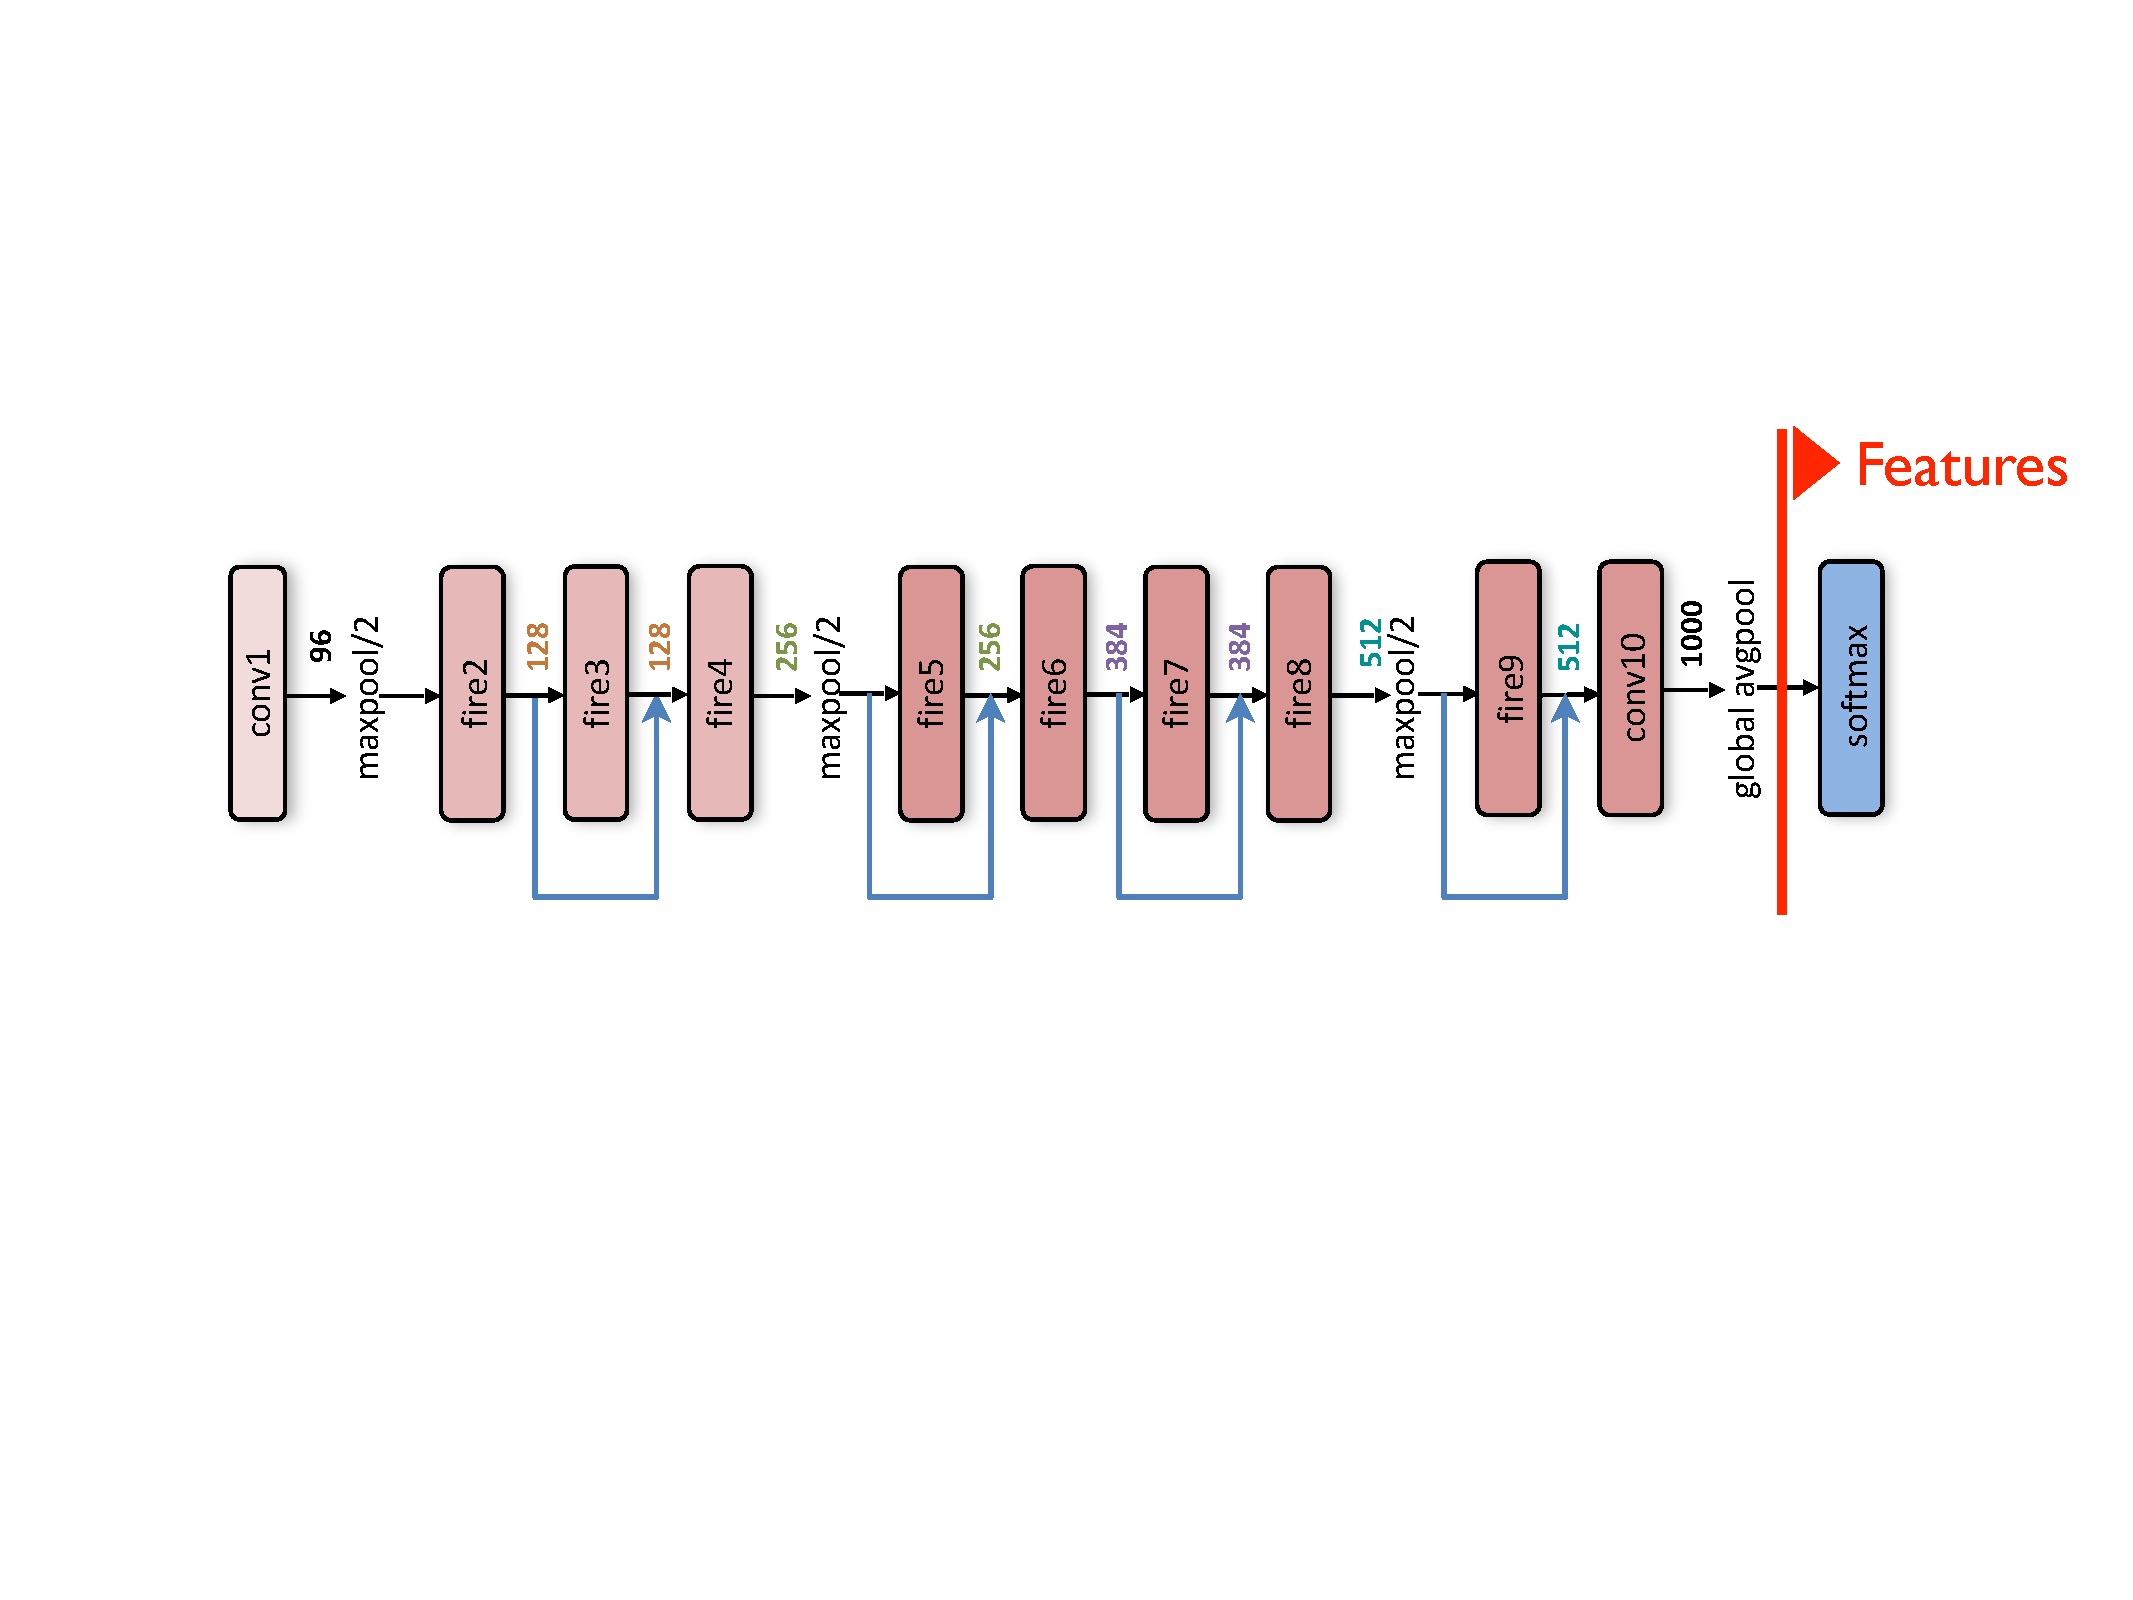
\includegraphics[width=0.95\textwidth]{../graphics/transfer_learning.pdf}
   \caption{Image representations for transfer learning. Image adapted from \cite{Iandola:2017}}
\end{figure}
\begin{itemize}
   \item Train a network on large annotated image bases.
   \item Use the learned representations to solve small scale problems (with or without fine-tuning) with few annotations.
   \item Problems:
   \begin{itemize}
   	\item Relevance of the used dataset.
   	\item Relevance of the tasks. 
   \end{itemize}
\end{itemize}
%\vspace{-.5cm}
\end{frame}


\begin{frame}{Subject of today}
In this lecture, we will learn about three strategies to address the problem of massive datasets required for training of deep neural networks:
\begin{enumerate}
\item Contrastive Learning
\item Learning in a weakly supervised setting (typically coarse annotations)
\item Learning from simulations with domain adaptation
\end{enumerate}
\end{frame}

%%%%%%%%%%%%%%%%%%%%%%%%%%%%%%%%%%%%%%%%%%%%%%%%%%%%%%%%%%%%%%%%%%%%%%%%%
%%%%%%%%%%%%%%%%%%%%%%%%%%%%%%%%%%%%%%%%%%%%%%%%%%%%%%%%%%%%%%%%%%%%%%%%%
\section{Contrastive Learning}
\frame{\frametitle{Overview}\tableofcontents[currentsection]}

\begin{frame}{Idea}
\begin{itemize}
%\item The success of Deep Learning in Computer Vision stems from the learning of good representations of the image data. 
%\item Idea: to use unlabeled data for representation learning.
\item Transfer Learning: transferring learned representation from one data set (with potentially different tasks) to a new data set. 
\item If we can define pretext tasks with known labels, we can also leverage unlabeled data to learn representations, which might also be transferable. 
\item Pretext task: learn the identity of transformed images. 
\item Here, we present the paper "A simple framework for Contrastive Learning of Visual Representations" (SimCLR) \cite{Chen2020}. 
\end{itemize}
\end{frame}

\begin{frame}{SimCLR \cite{Chen2020}}
\begin{figure}[htb]
   \centering
   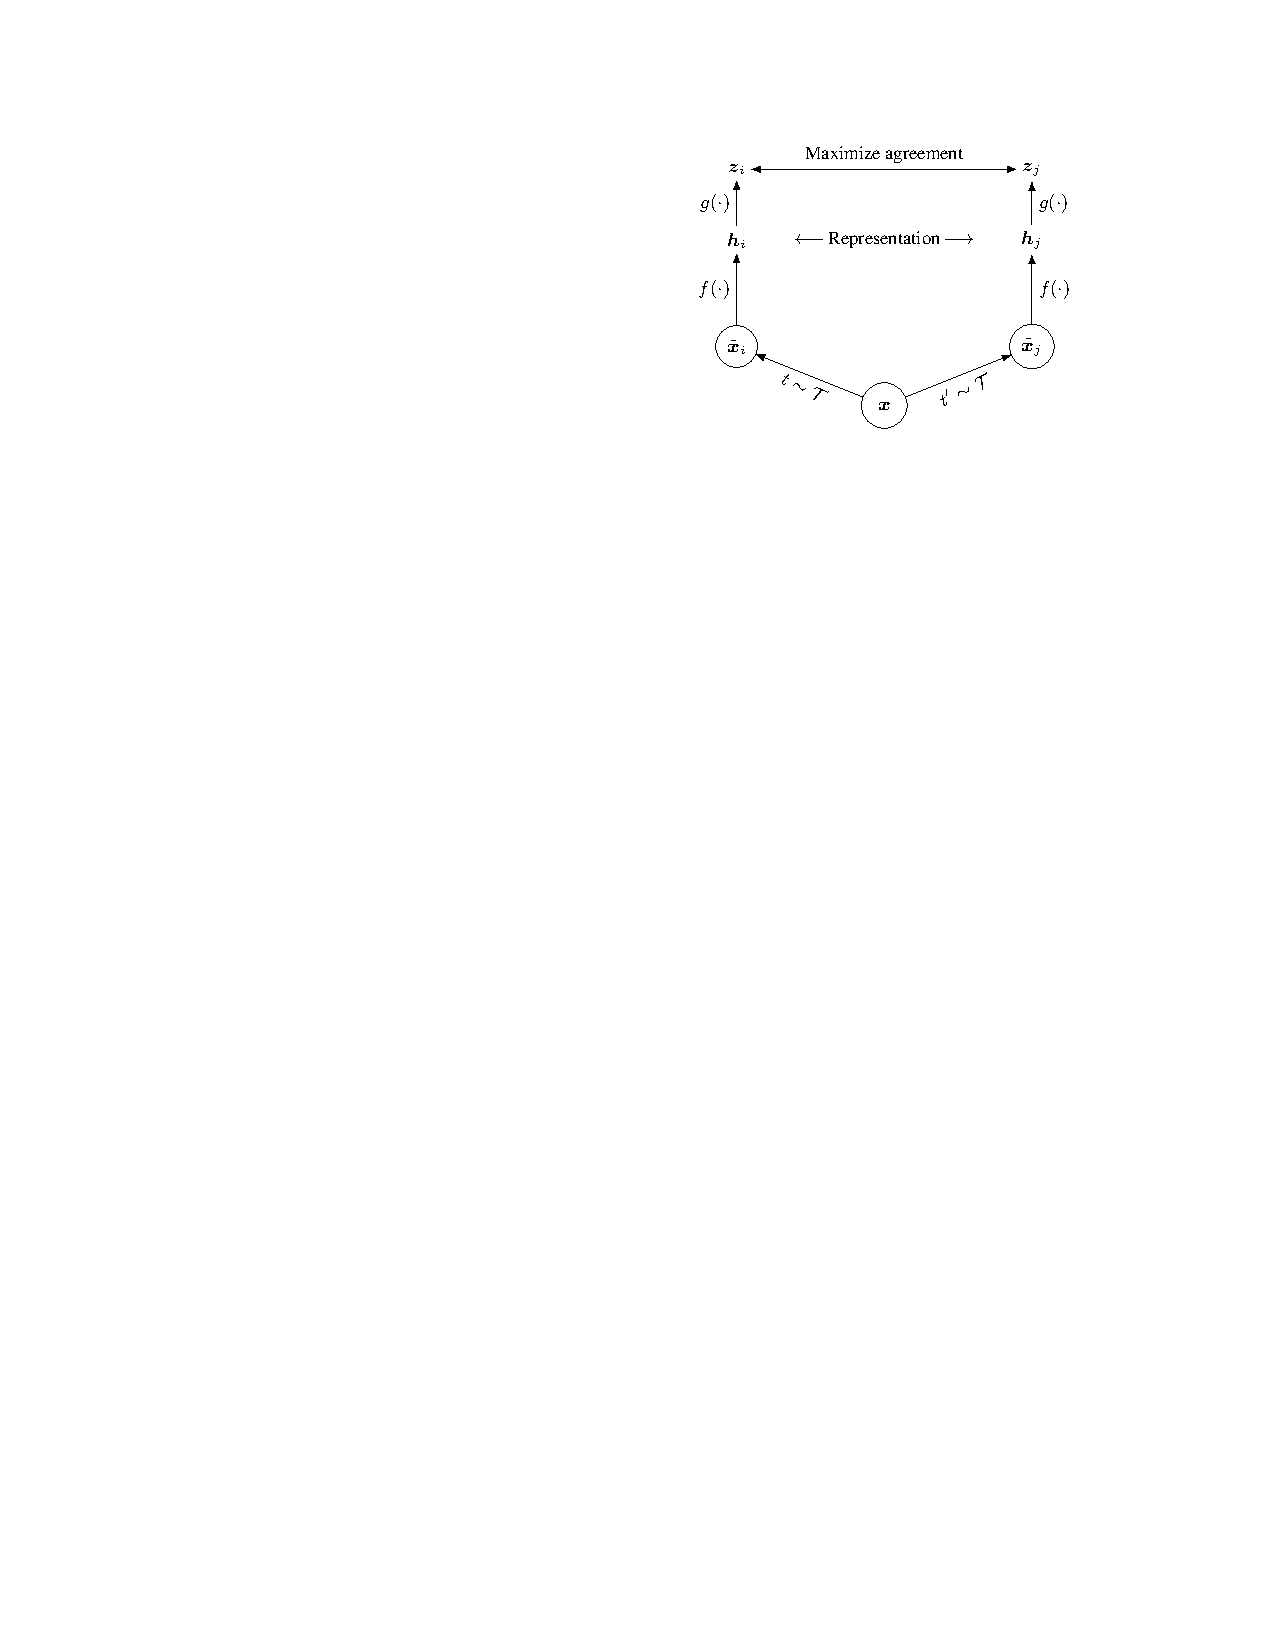
\includegraphics[height=0.4\textheight]{../graphics/sim_clr.pdf}
   \caption{SimCLR workflow as defined in \cite{Chen2020}}
\end{figure}
\begin{itemize}
\item For each image $x$, we calculate two transformed versions $\tilde{x}_i$ and $\tilde{x}_j$ by two transformations $t$ and $t'$ drawn from a set of parametrized transformations. 
%\begin{equation}
%\end{equation}
\item For $\tilde{x}_i$ and $\tilde{x}_j$, we calculate the representations $h_i$ and $h_j$, respectively. $f(\cdot)$ is the neural network we want to learn. 
\end{itemize}
\end{frame}

\begin{frame}{SimCLR \cite{Chen2020}}
\begin{figure}[htb]
   \centering
   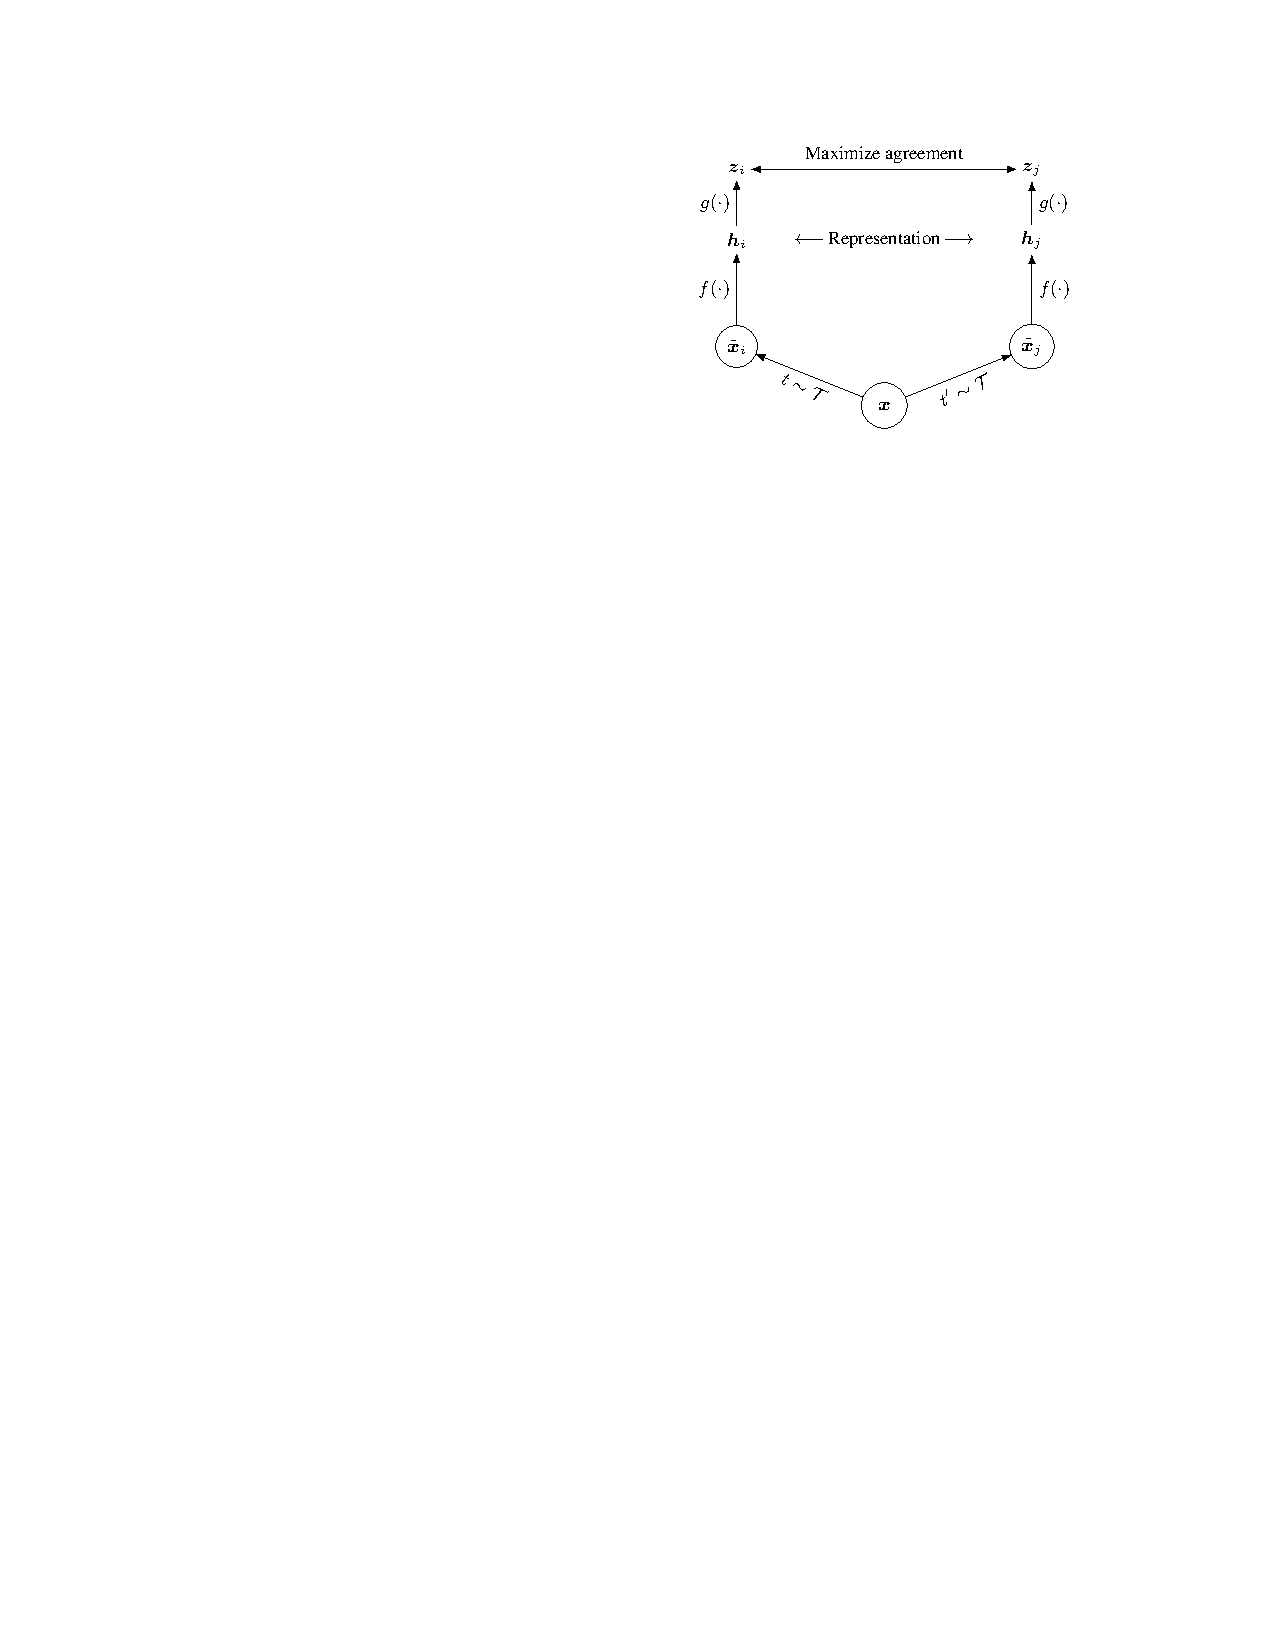
\includegraphics[width=0.4\textwidth]{../graphics/sim_clr.pdf}
   \caption{SimCLR workflow as defined in \cite{Chen2020}}
\end{figure}
\begin{itemize}
\item The representations $h_i$ and $h_j$ are mapped to a space where contrastive loss is applied, by a small neural network $g(\cdot)$. 
\item The classification task is to identify among all transformed images for each transformed image $x_i$ the transformed image $x_j$ that originates from the same image. 
\end{itemize}
\end{frame}

\begin{frame}{SimCLR \cite{Chen2020}}
\begin{figure}[htb]
   \centering
   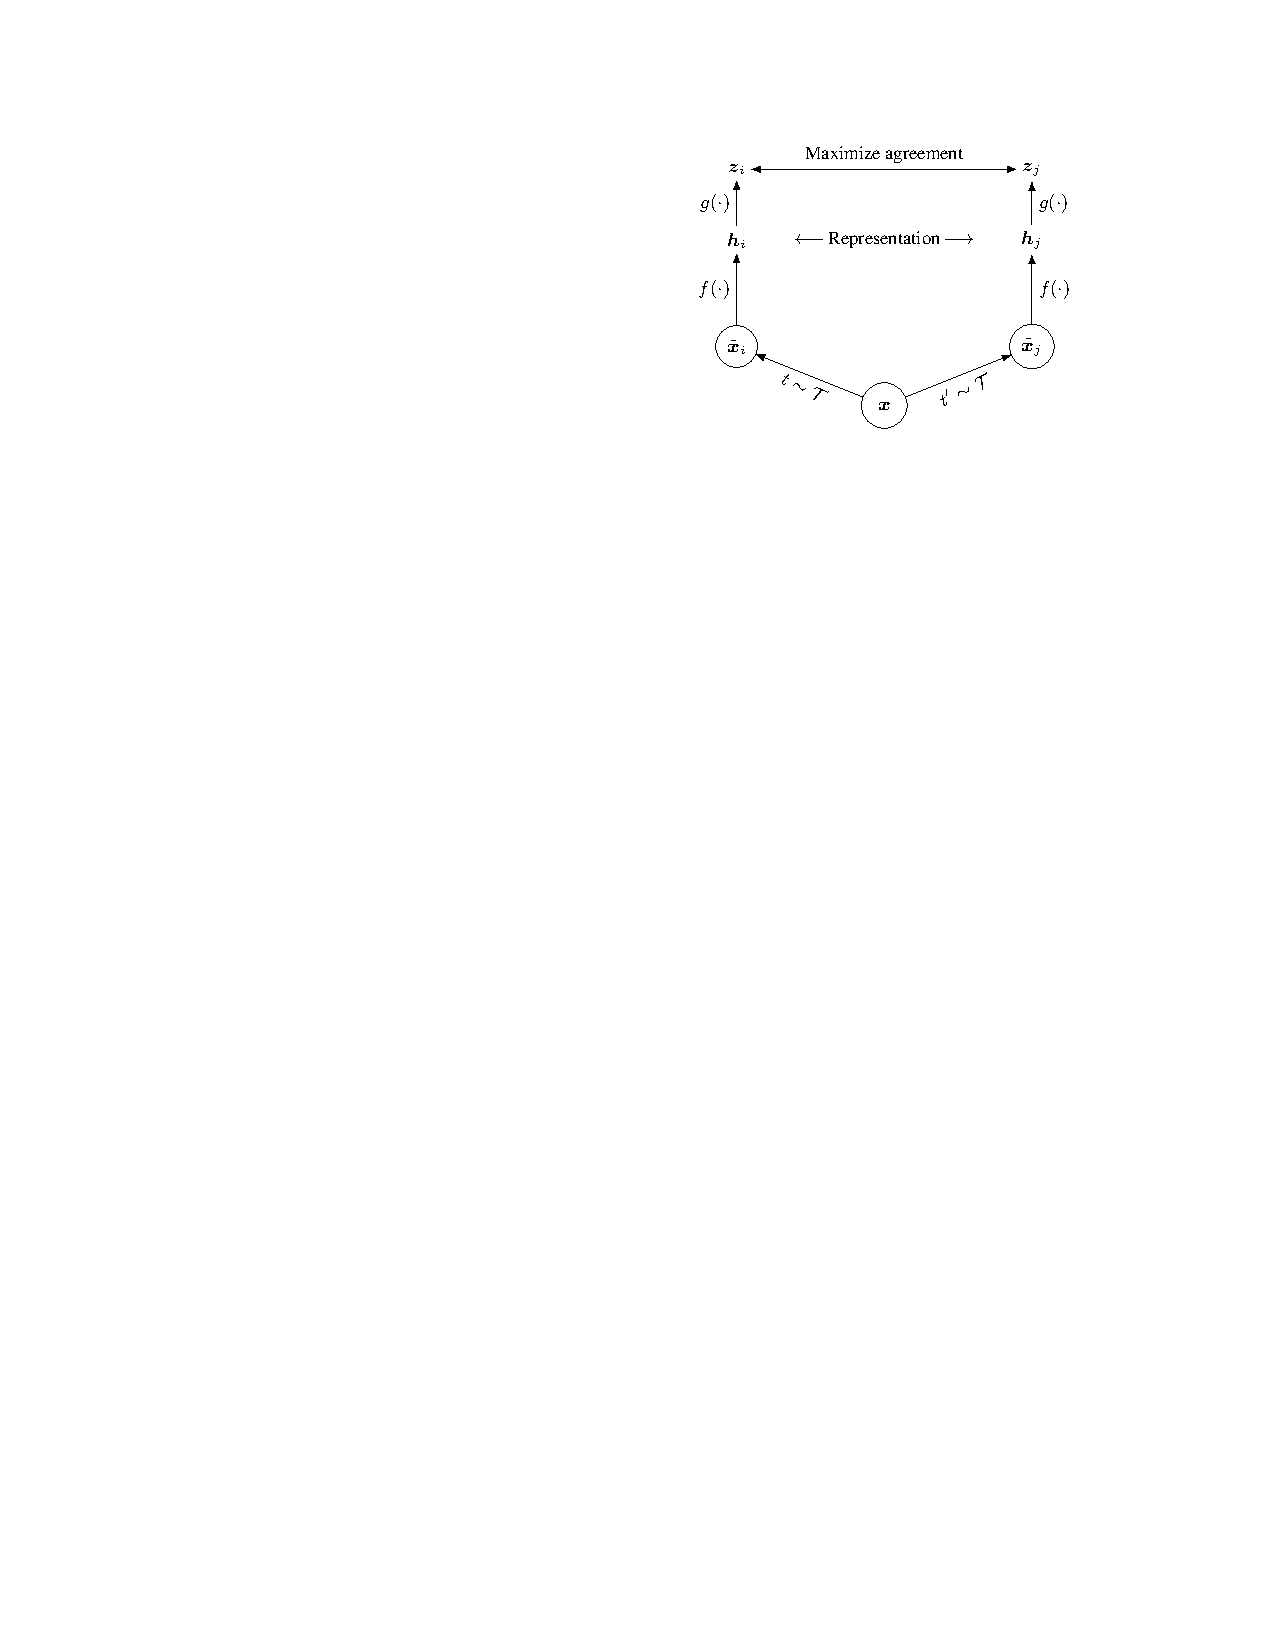
\includegraphics[width=0.4\textwidth]{../graphics/sim_clr.pdf}
   \caption{SimCLR workflow as defined in \cite{Chen2020}}
\end{figure}
\begin{itemize}
\item We define the similarity of two representations as follows:
\begin{equation}
s(u,v) = \frac{u^Tv}{\|u\|\|v\|}
\end{equation}
\item With this, we can define the contrastive loss as follows:
 \begin{equation}
 l_{i,j} = -\log \frac{\exp \frac{s(z_i, z_j)} {\tau}} {\sum_{k=1}^{2N}\vmathbb{1}_{k\neq i}\exp \frac{s(z_i, z_k)}{\tau} } 
\end{equation}
\end{itemize}
\end{frame}

\begin{frame}{SimCLR: transformations}
\begin{figure}[htb]
   \centering
   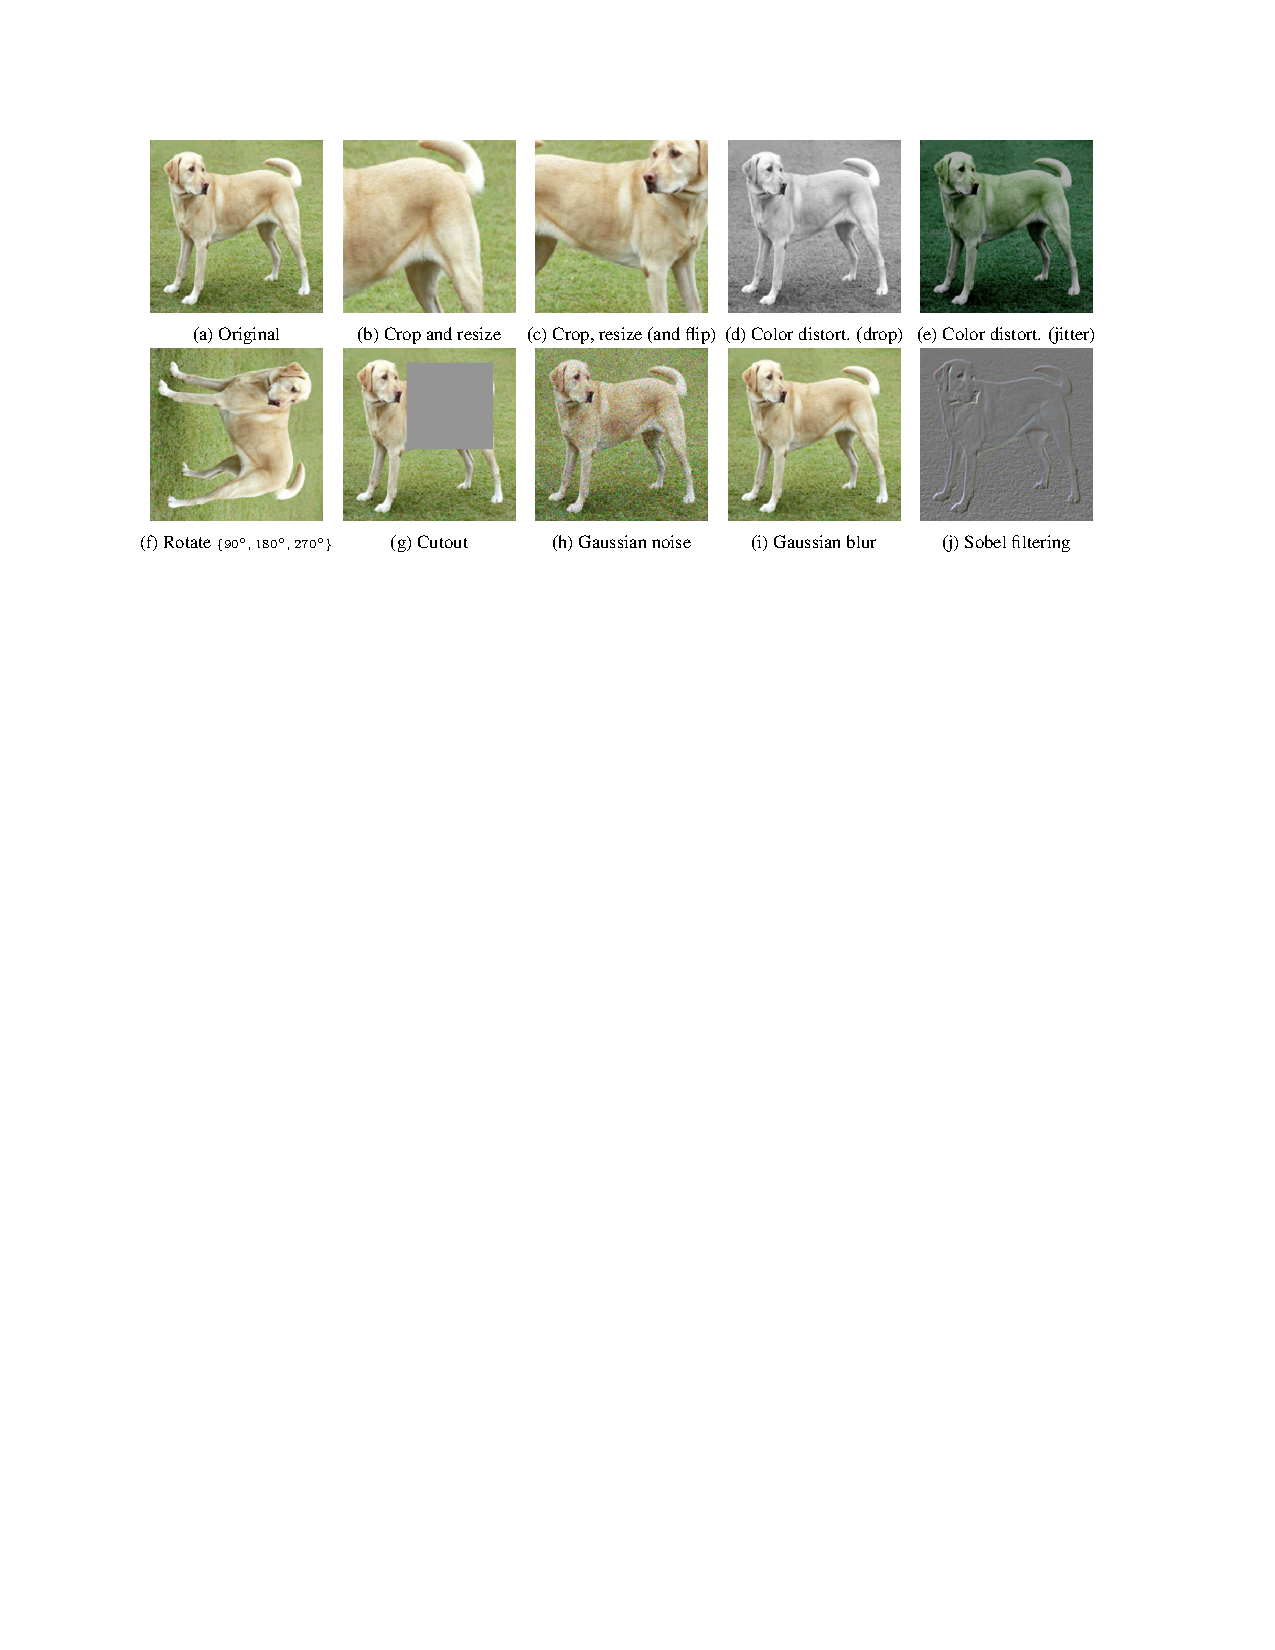
\includegraphics[width=0.9\textwidth]{../graphics/simclr_transformations.pdf}
   \caption{Transformations used in SimCLR \cite{Chen2020}}
\end{figure}
\end{frame}

\begin{frame}{SimCLR: results}
\begin{figure}[htb]
   \centering
   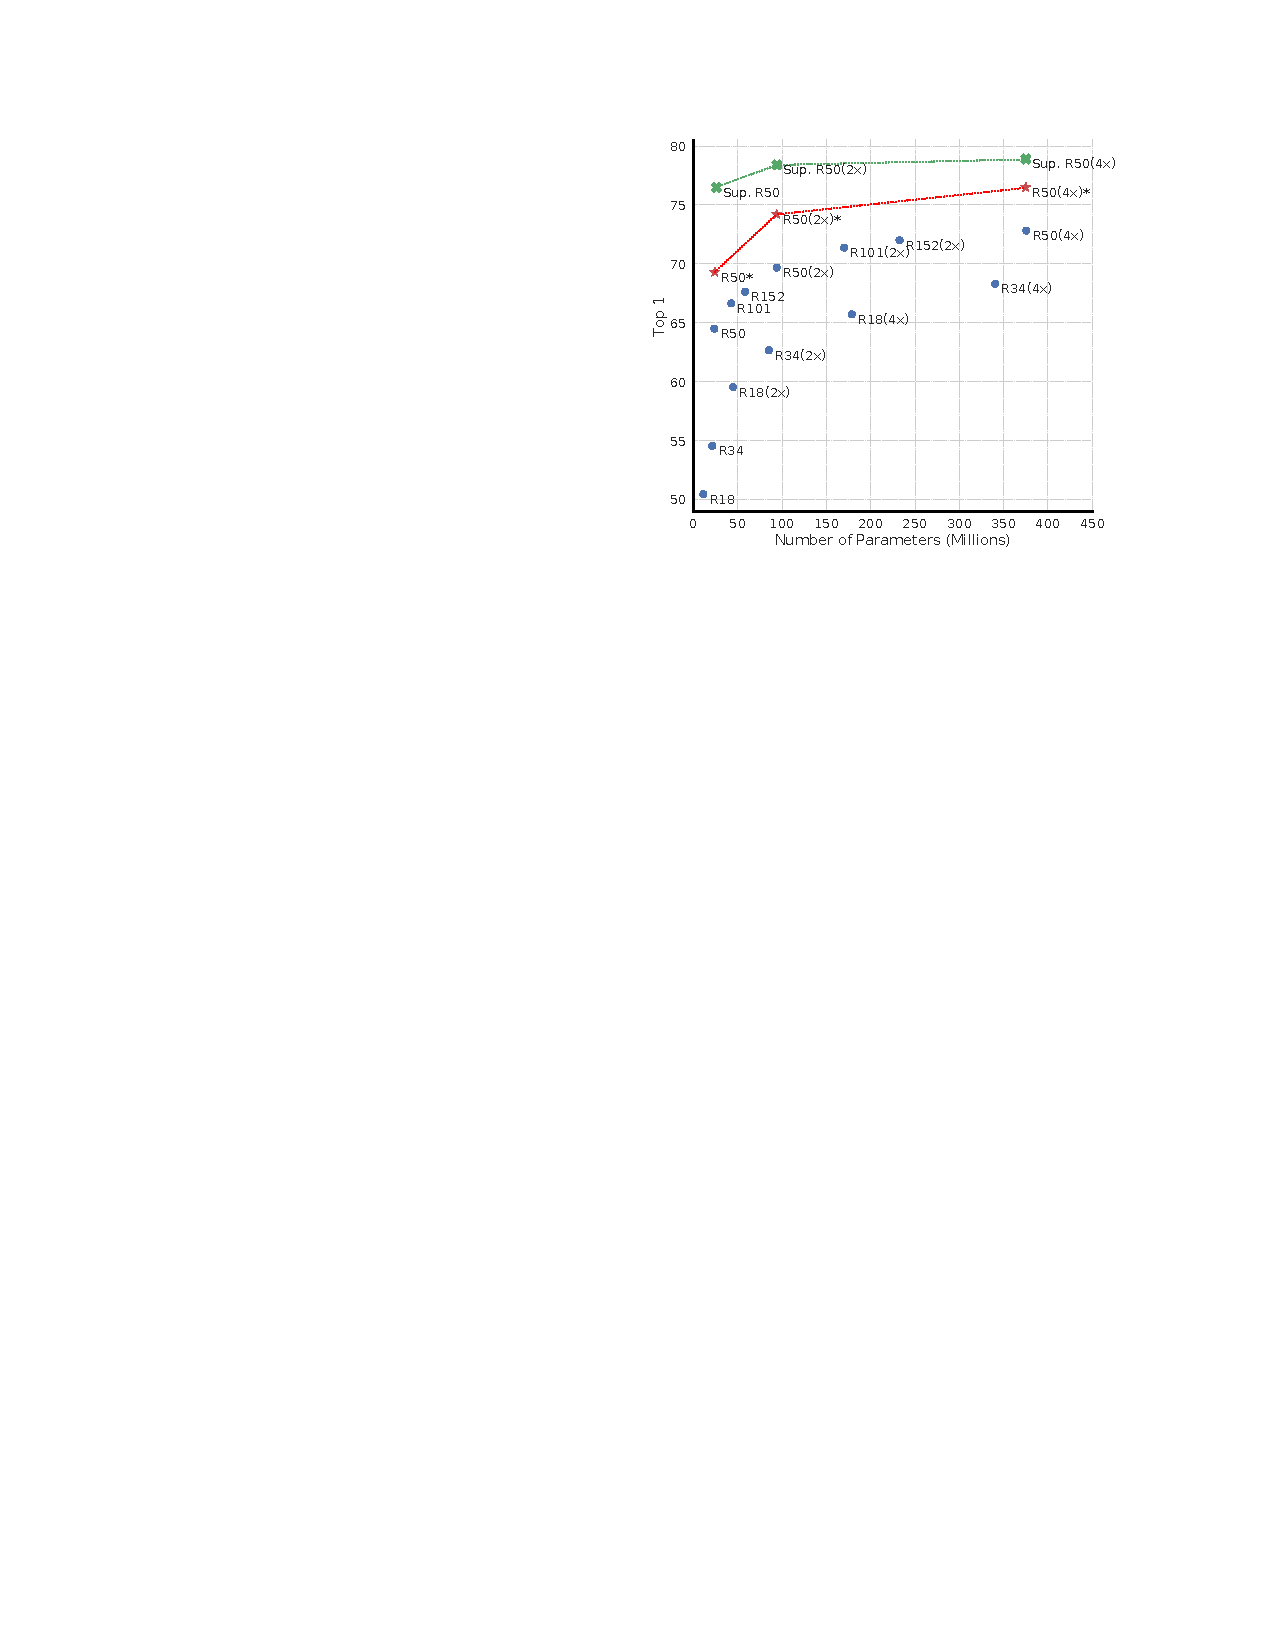
\includegraphics[width=0.4\textwidth]{../graphics/simclr_results.pdf}
   \caption{Results (linear evaluation) obtained by SimCLR \cite{Chen2020}}
\end{figure}
\begin{itemize}
\item Evaluation of representations by \emph{linear evaluation} (result obtained by a linear classifier trained with the representation as features): the unsupervised approach comes reasonably close to a fully supervised approach. 
\item Transfer-learning results (not shown): Fine-tuning the obtained representations is on par with fine-tuning pretrained networks. 
\end{itemize}
\end{frame}

%%%%%%%%%%%%%%%%%%%%%%%%%%%%%%%%%%%%%%%%%%%%%%%%%%%%%%%%%%%%%%%%%%%%%%%%%
%%%%%%%%%%%%%%%%%%%%%%%%%%%%%%%%%%%%%%%%%%%%%%%%%%%%%%%%%%%%%%%%%%%%%%%%%
\section{Weak supervision}
\frame{\frametitle{Overview}\tableofcontents[currentsection]}

\begin{frame}{What is weak supervision?}
\begin{itemize}
\item Weak supervision refers to a situation, where the ground truth data we build our model on is in some sense imperfect \cite{Zhou2018}. 
\item Three types of weak supervision:
\begin{enumerate}
\item \textbf{Incomplete supervision:} only a subset of training data are labeled (semisupervised setting).
\item \textbf{Inexact supervision:} training data are labeled but not as exactly as required by the task we would like to perform.
\item \textbf{Inaccurate supervision:} training data are labeled, but may contain mistakes. 
\end{enumerate}
\item Here, we treat the case of inexact supervision. 
\end{itemize}
\end{frame}

\begin{frame}{The Multiple Instance Learning framework (MIL)}
\begin{itemize}
\item MIL deals with problems with incomplete knowledge of labels in training sets.
\item MIL assumes that instead of disposing of individual labels $y_i$ for each sample $x_i$, we only have labels for subsets of samples, called "bags": 
\begin{eqnarray}
T &=& \{(B_i, y_i)\} \nonumber \\
B_i &=& \{x_j\}
\end{eqnarray}
\item A bag is positively labeled if at least one instance in it is positive, and is negatively labeled if all instances in it are negative.
\item Examples:
\begin{itemize}
   \item An image is labeled as "contains humans", if at least one region contains a human.
   \item A tissue slide is labeled cancerous, if at least one region is cancerous. 
\end{itemize}
\end{itemize}
\end{frame}

\begin{frame}{A deep learning approach to MIL}
\begin{figure}[htb]
   \centering
   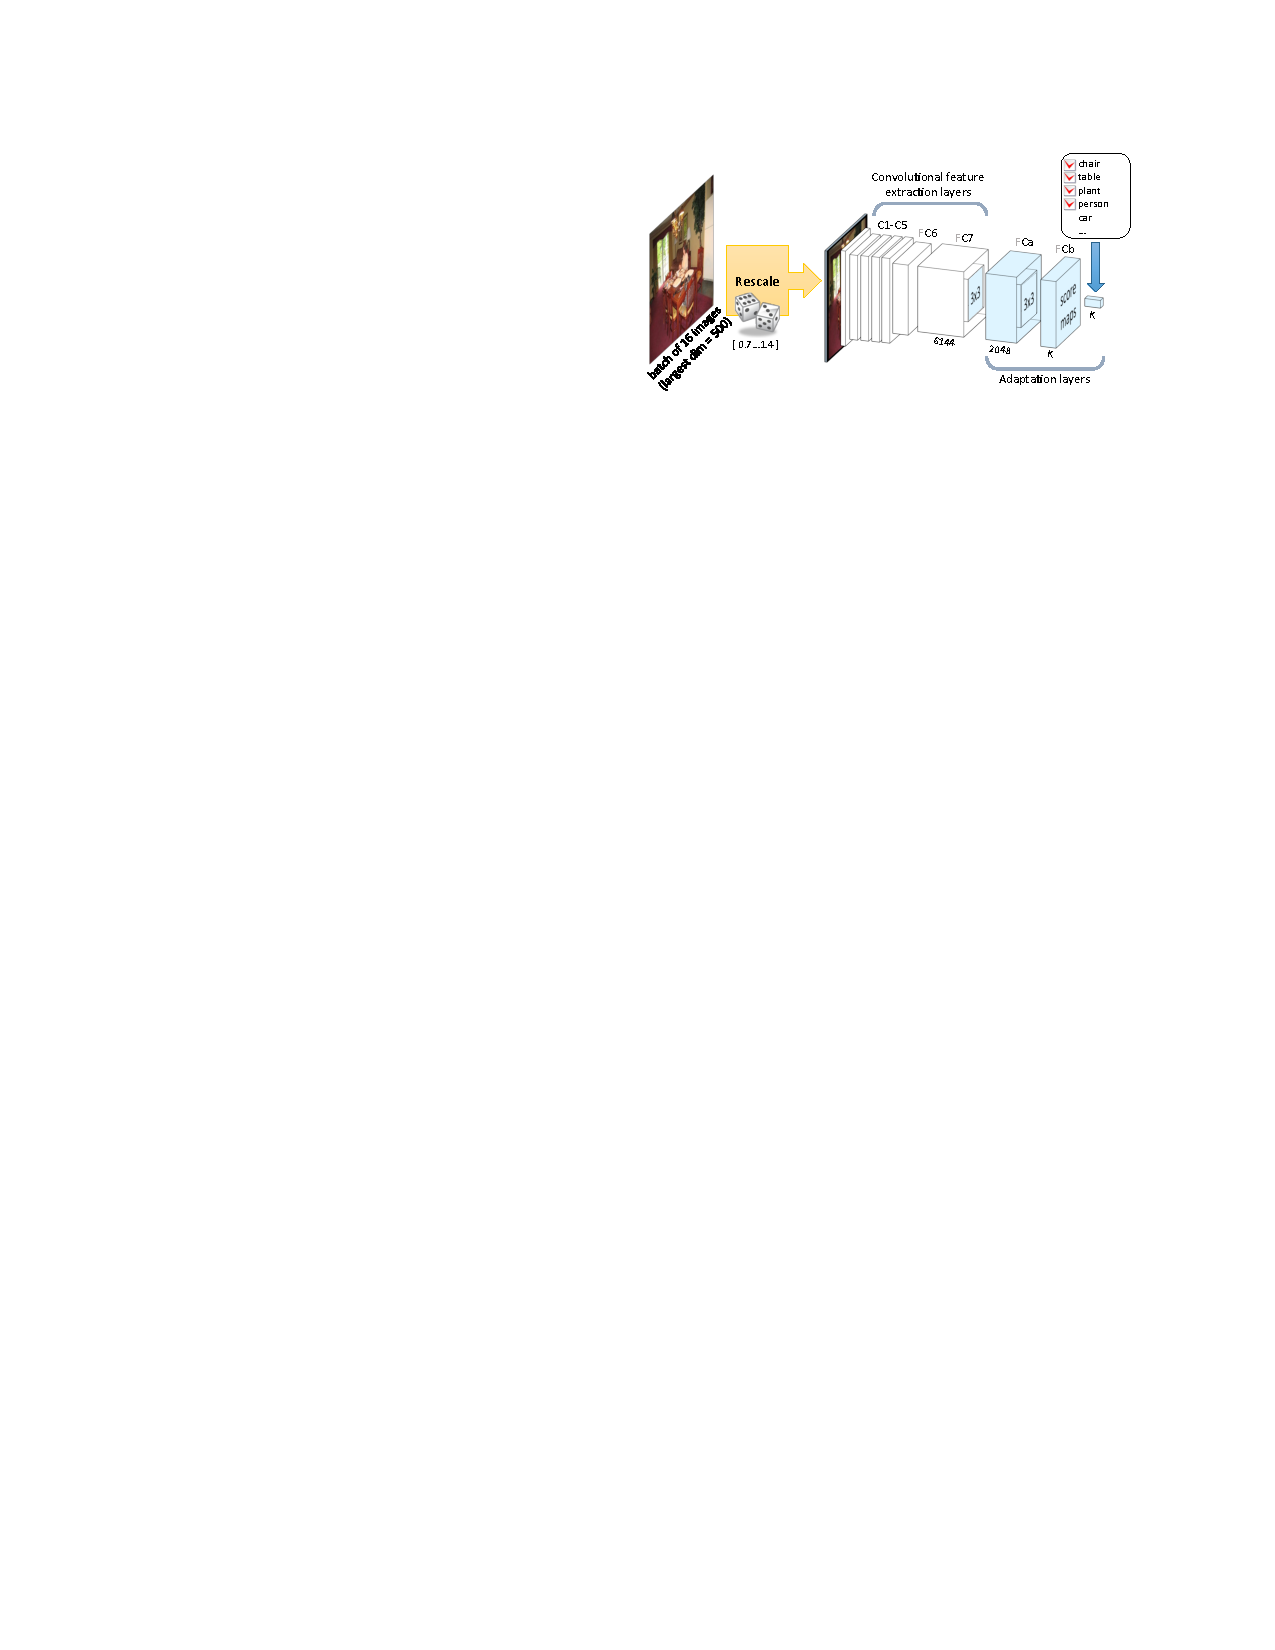
\includegraphics[width=0.9\textwidth]{../graphics/mil_deep_learning_v1.pdf}
   \caption{CNN architecture for Multiple Instance Learning. Image taken from \cite{Oquab2015}}
\end{figure}
First, a standard CNN is applied as feature extractor (without fully connected layers). This maps an image $X$ to a $n \times m \times l$ layer ($l$ feature maps of spatial dimensions $n \times m$). 
\end{frame}

\begin{frame}[noframenumbering]{A deep learning approach to MIL}
\begin{figure}[htb]
   \centering
   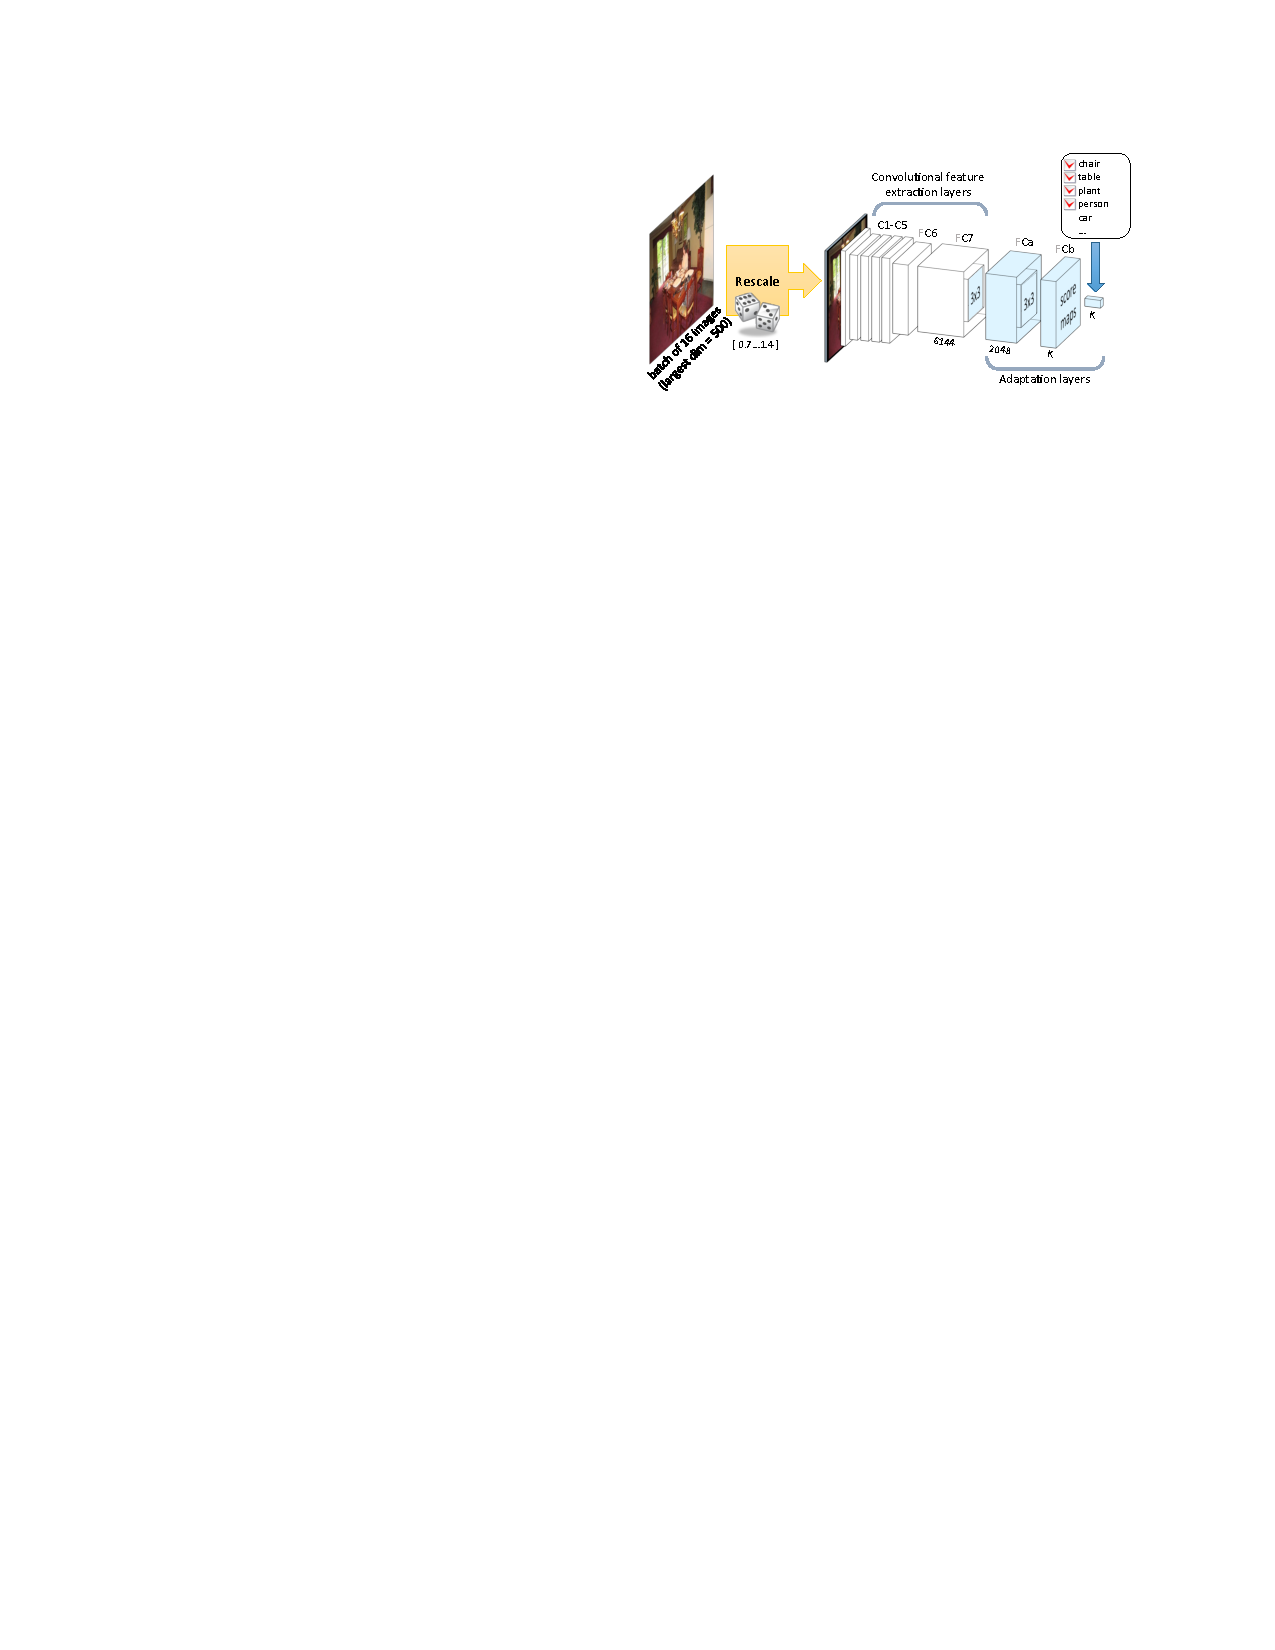
\includegraphics[width=0.9\textwidth]{../graphics/mil_deep_learning_v1.pdf}
   \caption{CNN architecture for Multiple Instance Learning. Image taken from \cite{Oquab2015}}
\end{figure}
This layer is then mapped to a $n \times m \times K$ layer by $1 \times 1$ convolutions, where $K$ is the number of output classes. Of note, a $1 \times 1$ convolutional layer is equivalent to a fully connected layer, if its input is a vector (spatial dimension 1). We can understand the $1 \times 1$ conv layer as parallel fully connected layers. 
%If the input has spatial dimensions $n \times m$, this corresponds to $nm$ independent fully connected layers. 
\end{frame}

\begin{frame}[noframenumbering]{A deep learning approach to MIL}
\begin{figure}[htb]
   \centering
   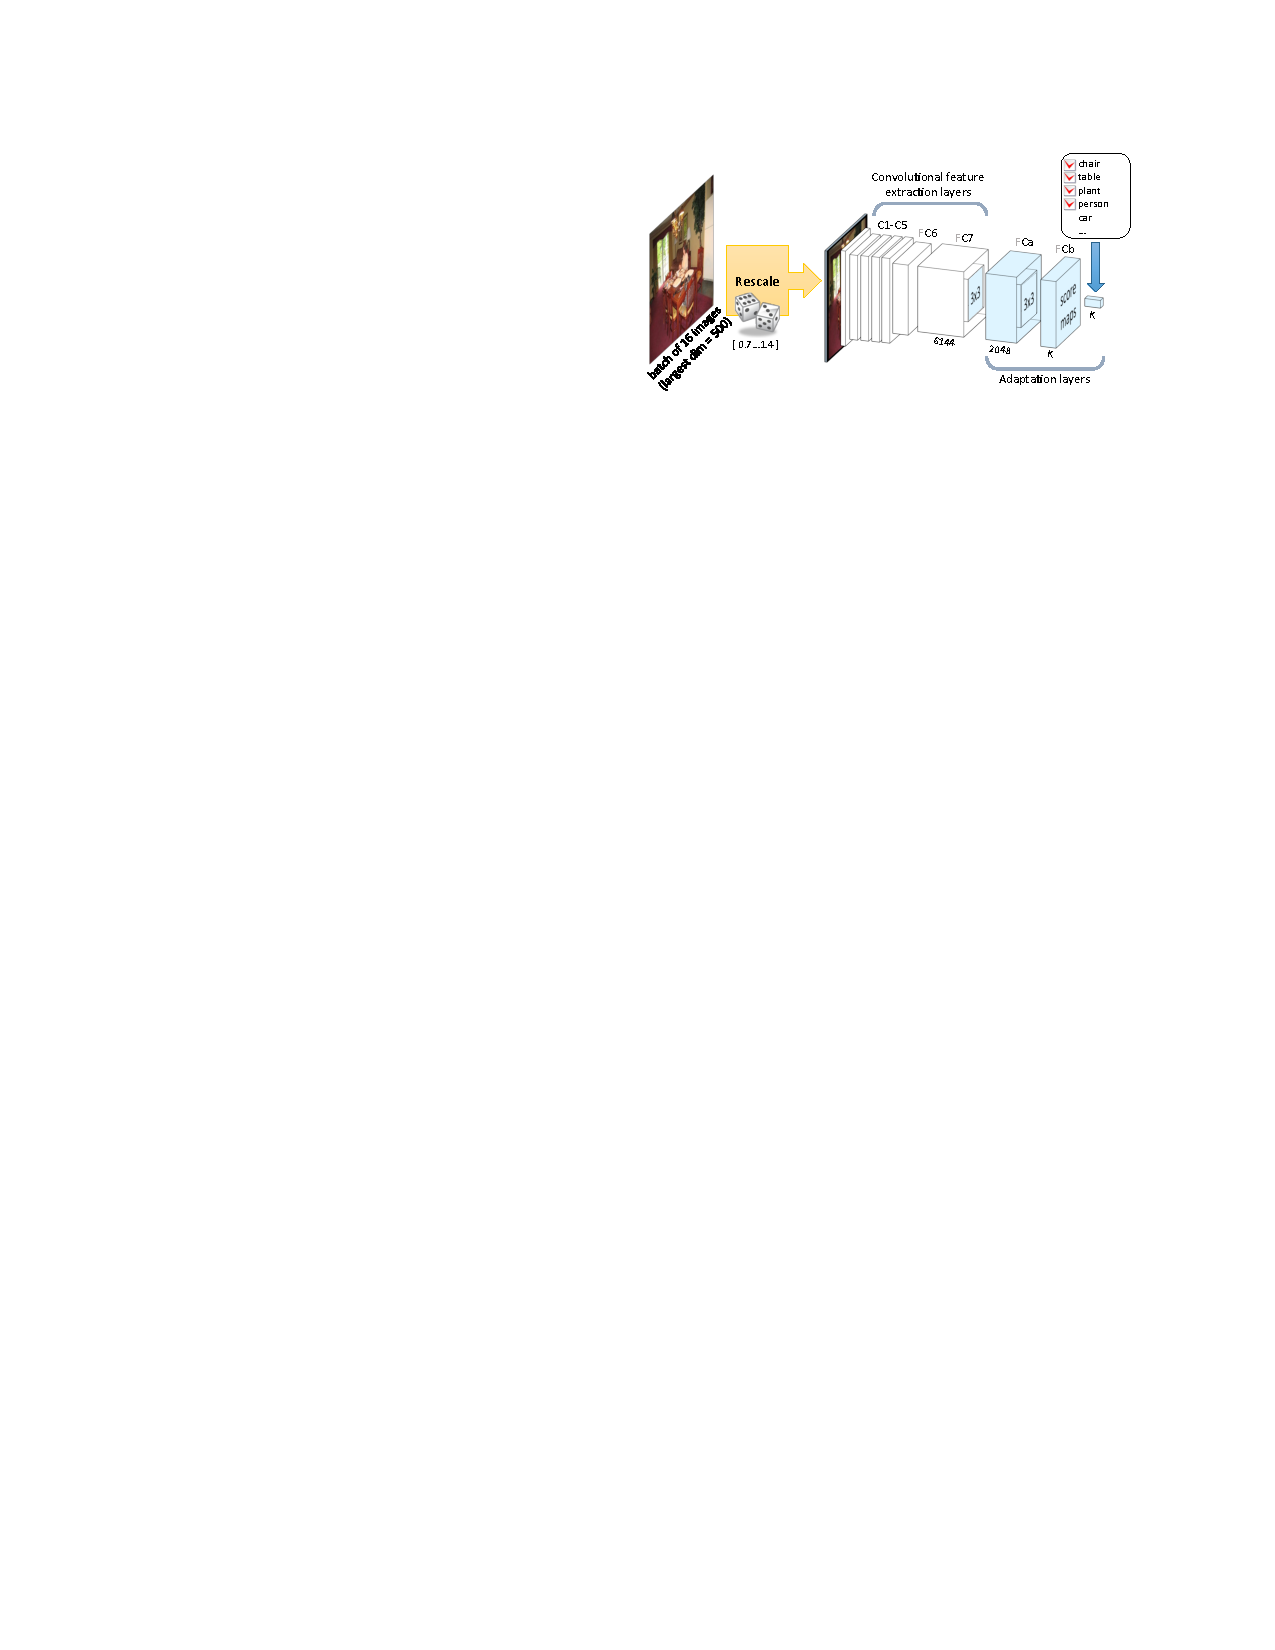
\includegraphics[width=0.9\textwidth]{../graphics/mil_deep_learning_v1.pdf}
   \caption{CNN architecture for Multiple Instance Learning. Image taken from \cite{Oquab2015}}
\end{figure}
Each "pixel" in feature map $FCb$ is thus the score vector for an input region. $FCb$ therefore corresponds to a bag of image regions. We therefore maximize over the spatial dimensions:
\begin{equation}
   s_k = \max_{i,j}f_{i,j}^k
\end{equation}
\end{frame}

\begin{frame}{A deep learning approach to MIL}
\begin{figure}[htb]
   \centering
   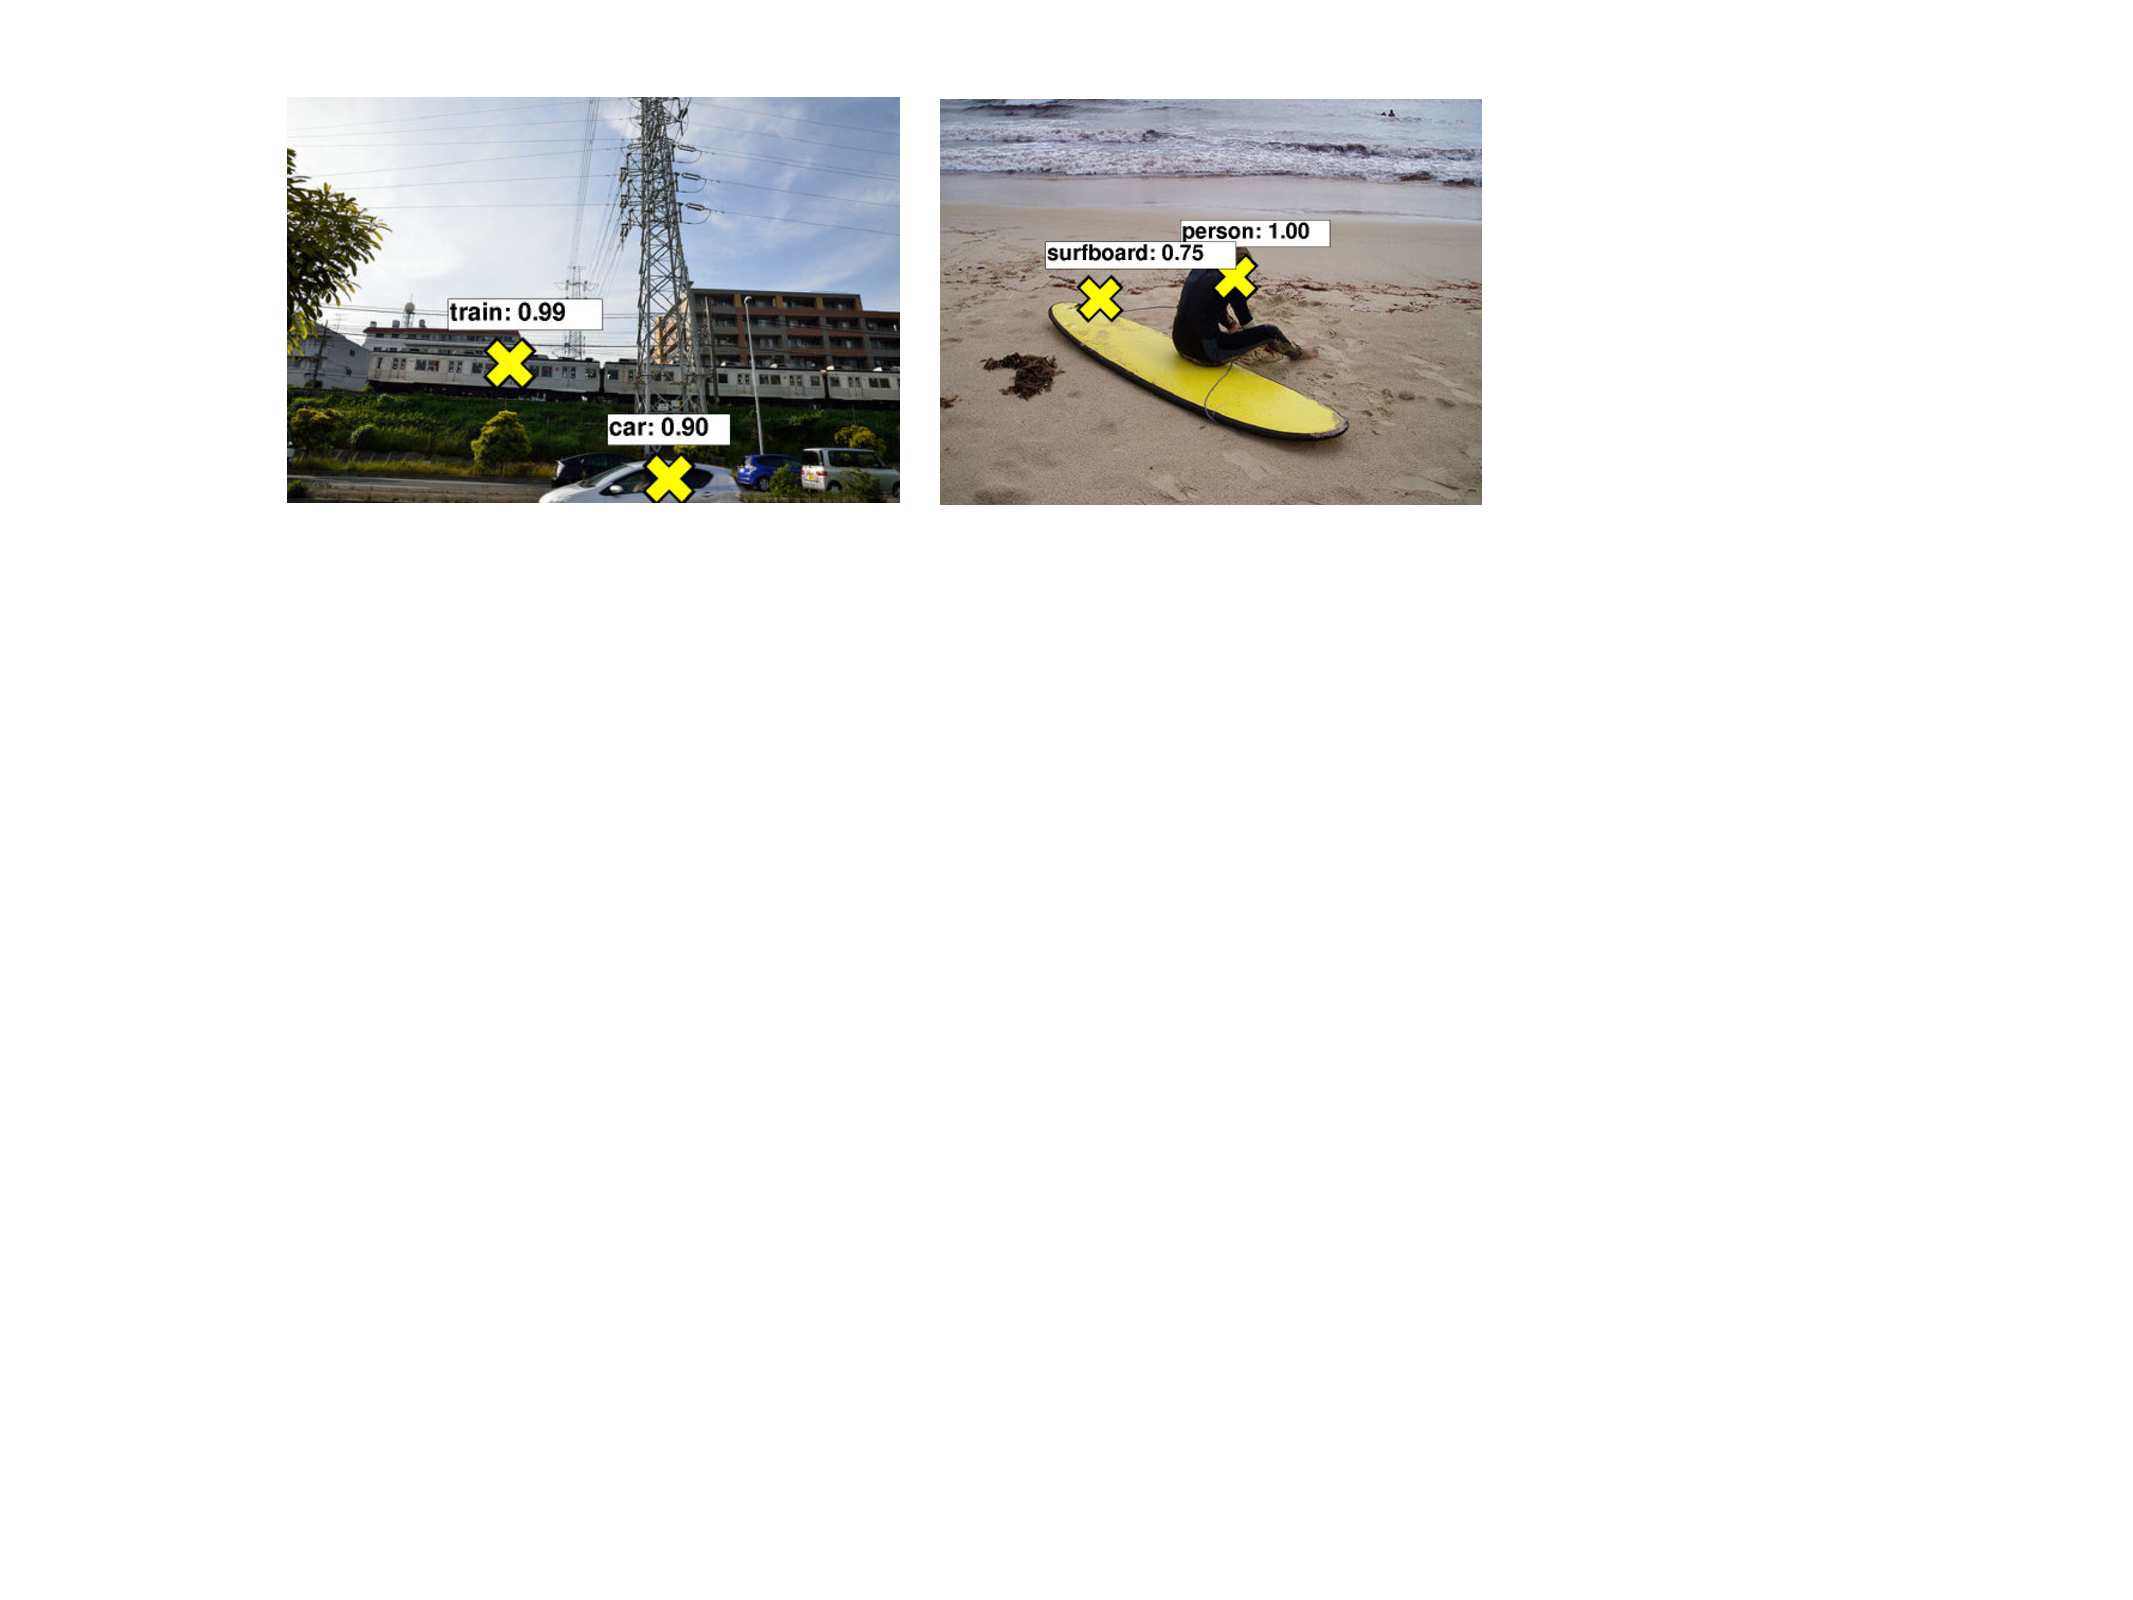
\includegraphics[width=0.7\textwidth]{../graphics/example_res_simple_wsl.pdf}
   \caption{Example for MIL by deep learning. Image adapted from \cite{Oquab2015}}
\end{figure}
\begin{itemize}
\item Maximization over the spatial dimensions corresponds exactly to the MIL-paradigm: for the decision on the image label, it is sufficient to have one single positive region. 
\item This is a typical situation, when we want to detect objects in crowded images. 
\end{itemize}
\end{frame}

% % the loss
% \begin{frame}{Co-existence of several objects}
% \begin{itemize}
% \item In this kind of WSL setting, each image can have several labels. 
% \item In this case, the softmax is not an optimal choice as output layer: classes are not mutually exclusive. 
% \item We can then simply take the sigmoid of the output scores:
% \end{itemize}
% \end{frame}

\begin{frame}{Discussion}
\begin{itemize}
   \item Improvement of image classification, as only the relevant region is taken into consideration.
   \item This is particularly useful, if the size of the relevant region is comparatively small. 
   \item Objects can also be detected and this without expensive annotation (bounding boxes or pixel-wise annotation). 
   \item In addition, the detection of different classes is eased by the setup. 
   \item Limitations:
   \begin{itemize}
      \item The max-operation might lead to instabilities.
      \item Object extensions cannot be faithfully predicted. 
      \item The context is not taken into consideration. 
   \end{itemize}
\end{itemize}
\end{frame}

\begin{frame}{Improvements on the WSL strategy}
\begin{itemize}
   \item Instead of taking the maximum score over all image regions \cite{Durand2016}:
   \begin{itemize}
      \item Select the $s_{top}$ highest scoring regions
      \item Select the $s_{low}$ lowest scoring regions
   \end{itemize}
   \item Intuition: taking $s_{top}>1$ regions makes the algorithm more robust, taking $s_{low}$ lowest scoring regions provides negative evidence for the class. 
\end{itemize}
\end{frame}

\begin{frame}{Application example: histopathology}
\begin{figure}[htb]
   \centering
   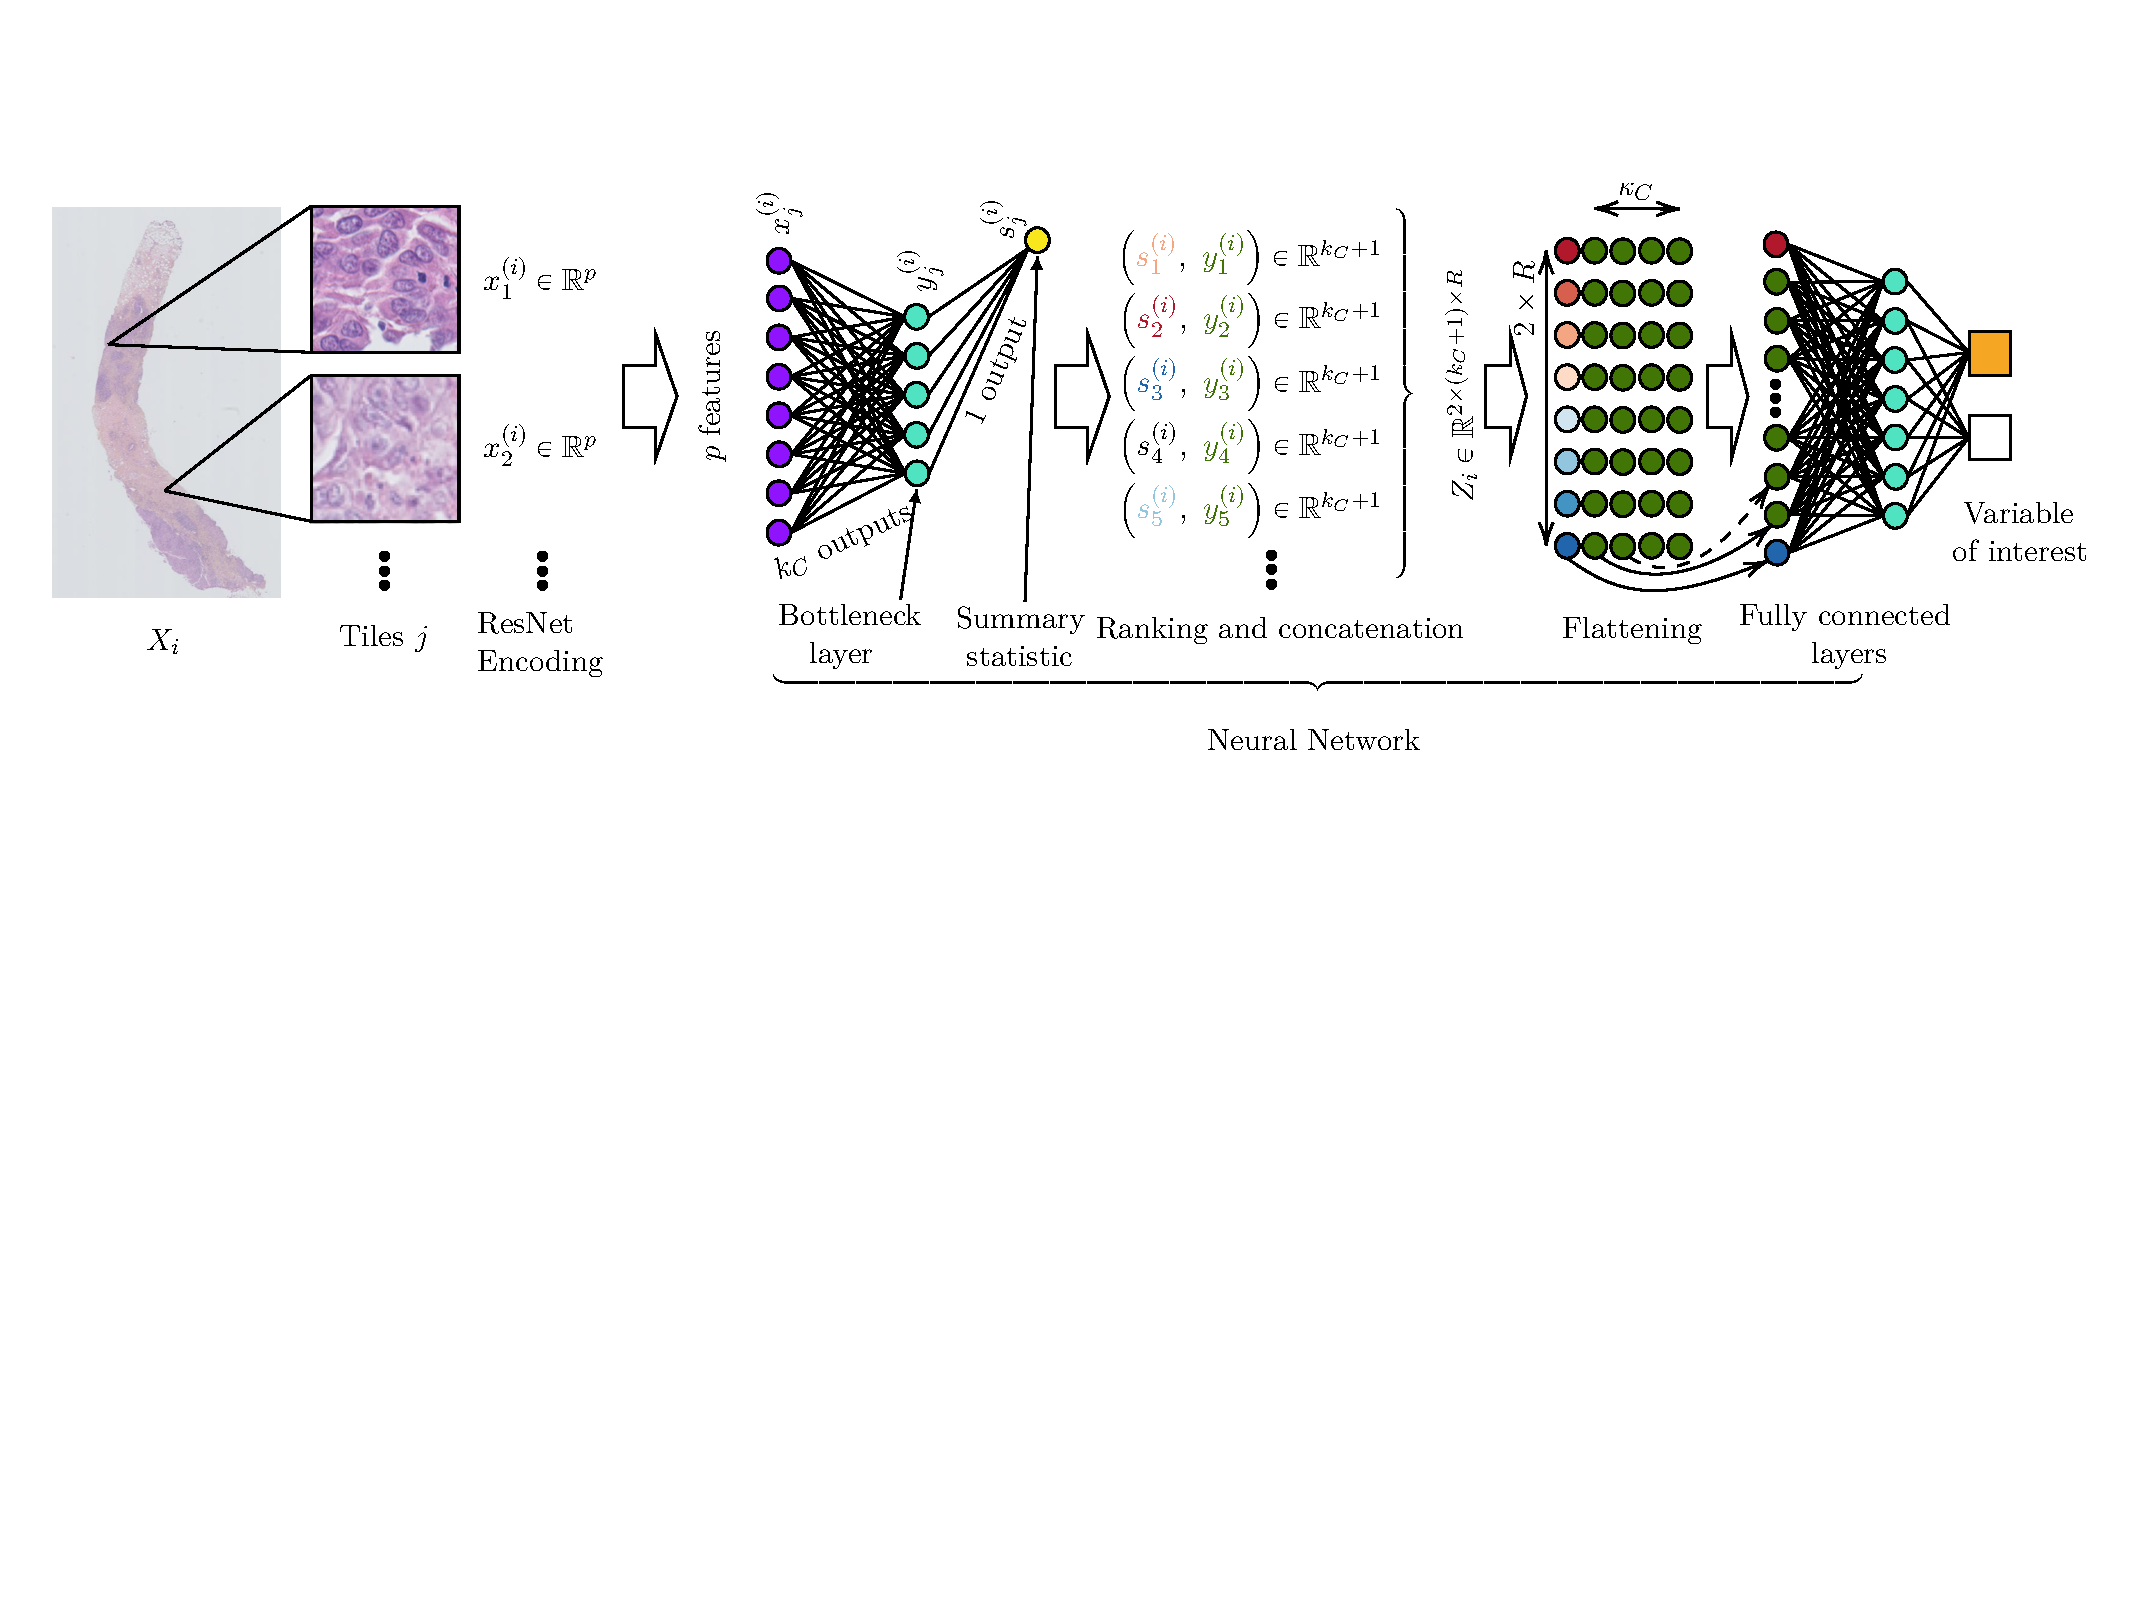
\includegraphics[width=0.9\textwidth]{../graphics/wsl_histo.pdf}
   \caption{Example for WSL for tumor detection. Image provided by Peter Naylor.}
\end{figure}
\begin{itemize}
\item Histopathology images are extremely big.
\item Sometimes, what we want to find can be small.
\item There is slide-level annotation, but detailed annotation is scarce.
\end{itemize}
\end{frame}


\begin{frame}{Application example: metastasis detection}
\begin{figure}[htb]
   \centering
   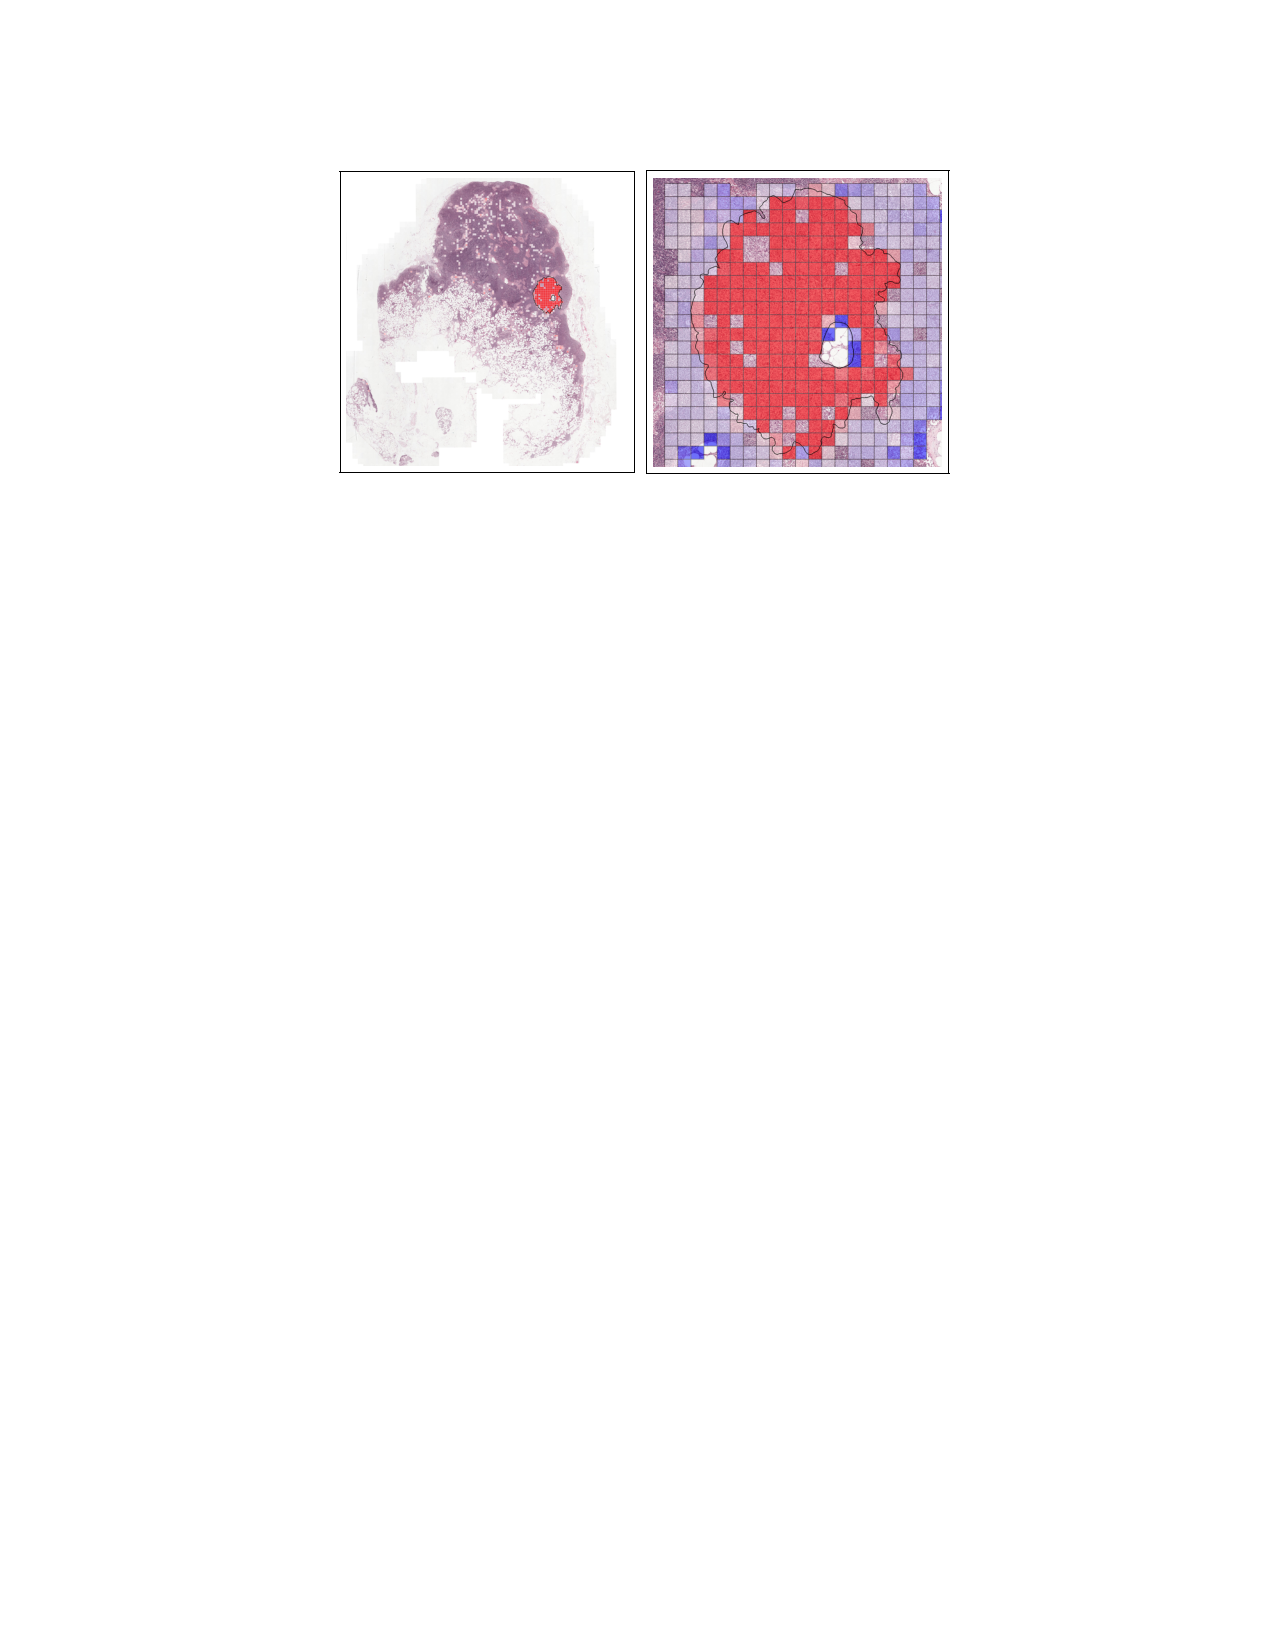
\includegraphics[width=0.6\textwidth]{../graphics/wsl_example_histopathology.pdf}
   \caption{Example for WSL for tumor detection. Image adapted from \cite{courtiolClassificationDiseaseLocalization2017}}
\end{figure}
Here, \cite{courtiolClassificationDiseaseLocalization2017} use the WELDON algorithm to detect metastases. Only global annotation is used. The results are on par with classification / detection algorithms trained on detailed annotation. 
\end{frame}


%%%%%%%%%%%%%%%%%%%%%%%%%%%%%%%%%%%%%%%%%%%%%%%%%%%%%%%%%%%%%%%%%%%%%%%%%
%%%%%%%%%%%%%%%%%%%%%%%%%%%%%%%%%%%%%%%%%%%%%%%%%%%%%%%%%%%%%%%%%%%%%%%%%
\section{Learning from simulated data}
\frame{\frametitle{Overview}\tableofcontents[currentsection]}

\begin{frame}{Simulation for the generation of training data}
\begin{itemize}
\item With simulation, we can generate arbitrary quantities of data with known ground truth. 
\item Simulation is regularly used for benchmarking of methods.
%\item Many different techniques: physical simulation, statistical simulation, 
\item Usually, simulation provides us with data similar to real world data, but not identical. 
\item For this reason, the use of simulated data for training neural networks is limited. 
\item Idea: can we overcome the differences between simulated and real data by explicit algorithmic strategies? 
\end{itemize}
\end{frame}

% Learning a discriminative classifier or other predictor in the presence of a shift be- tween training and test distributions is known as domain adaptation (DA). The proposed approaches build mappings between the source (training-time) and the target (test-time) domains, so that the classifier learned for the source domain can also be applied to the target domain, when composed with the learned mapping between domains.

% We consider classification tasks where X is the input space and Y = {0, 1, . . . , L−1} is the
% set of L possible labels. Moreover, we have two different distributions over X×Y , called the
% source domain DS and the target domain DT. An unsupervised domain adaptation learning
% algorithm is then provided with a labeled source sample S drawn i.i.d. from DS, and an
% unlabeled target sample T drawn i.i.d. from DX , where DX is the marginal distribution of TT
% DT over X.

\begin{frame}{Domains}
\begin{itemize}
\item Domain adaptation: learning a discriminative classifier when training data does not follow the same distribution as the test data.
\item Let $\mathcal{X}$ be an input space and $\mathcal{Y} = \{ 1, \ldots, L\}$ the set of $L$ possible labels. We call a domain the distribution over $\mathcal{X} \times \mathcal{Y}$. 
\item Here we consider two domains: the source domain $\mathcal{D}_S$ and the target domain $\mathcal{D}_T$. 
\item The $n$ source samples are then drawn from $\mathcal{D}_S$, the $N-n$ test samples from $\mathcal{D}_T$: 
\begin{eqnarray}
S &=& \{(x_i, y_i)\}_{i=1}^n \sim \mathcal{D}_S^n \nonumber \\
T &=& \{(x_i, y_i)\}_{i=n+1}^N \sim \mathcal{D}^{N-n}_T \nonumber 
\end{eqnarray}
%where $\mathcal{D}^X_T$ is the marginal distribution of $\mathcal{D}_T$. 
\end{itemize}
\end{frame}

\begin{frame}{The divergence of domains}
\begin{figure}[htb]
   \centering
   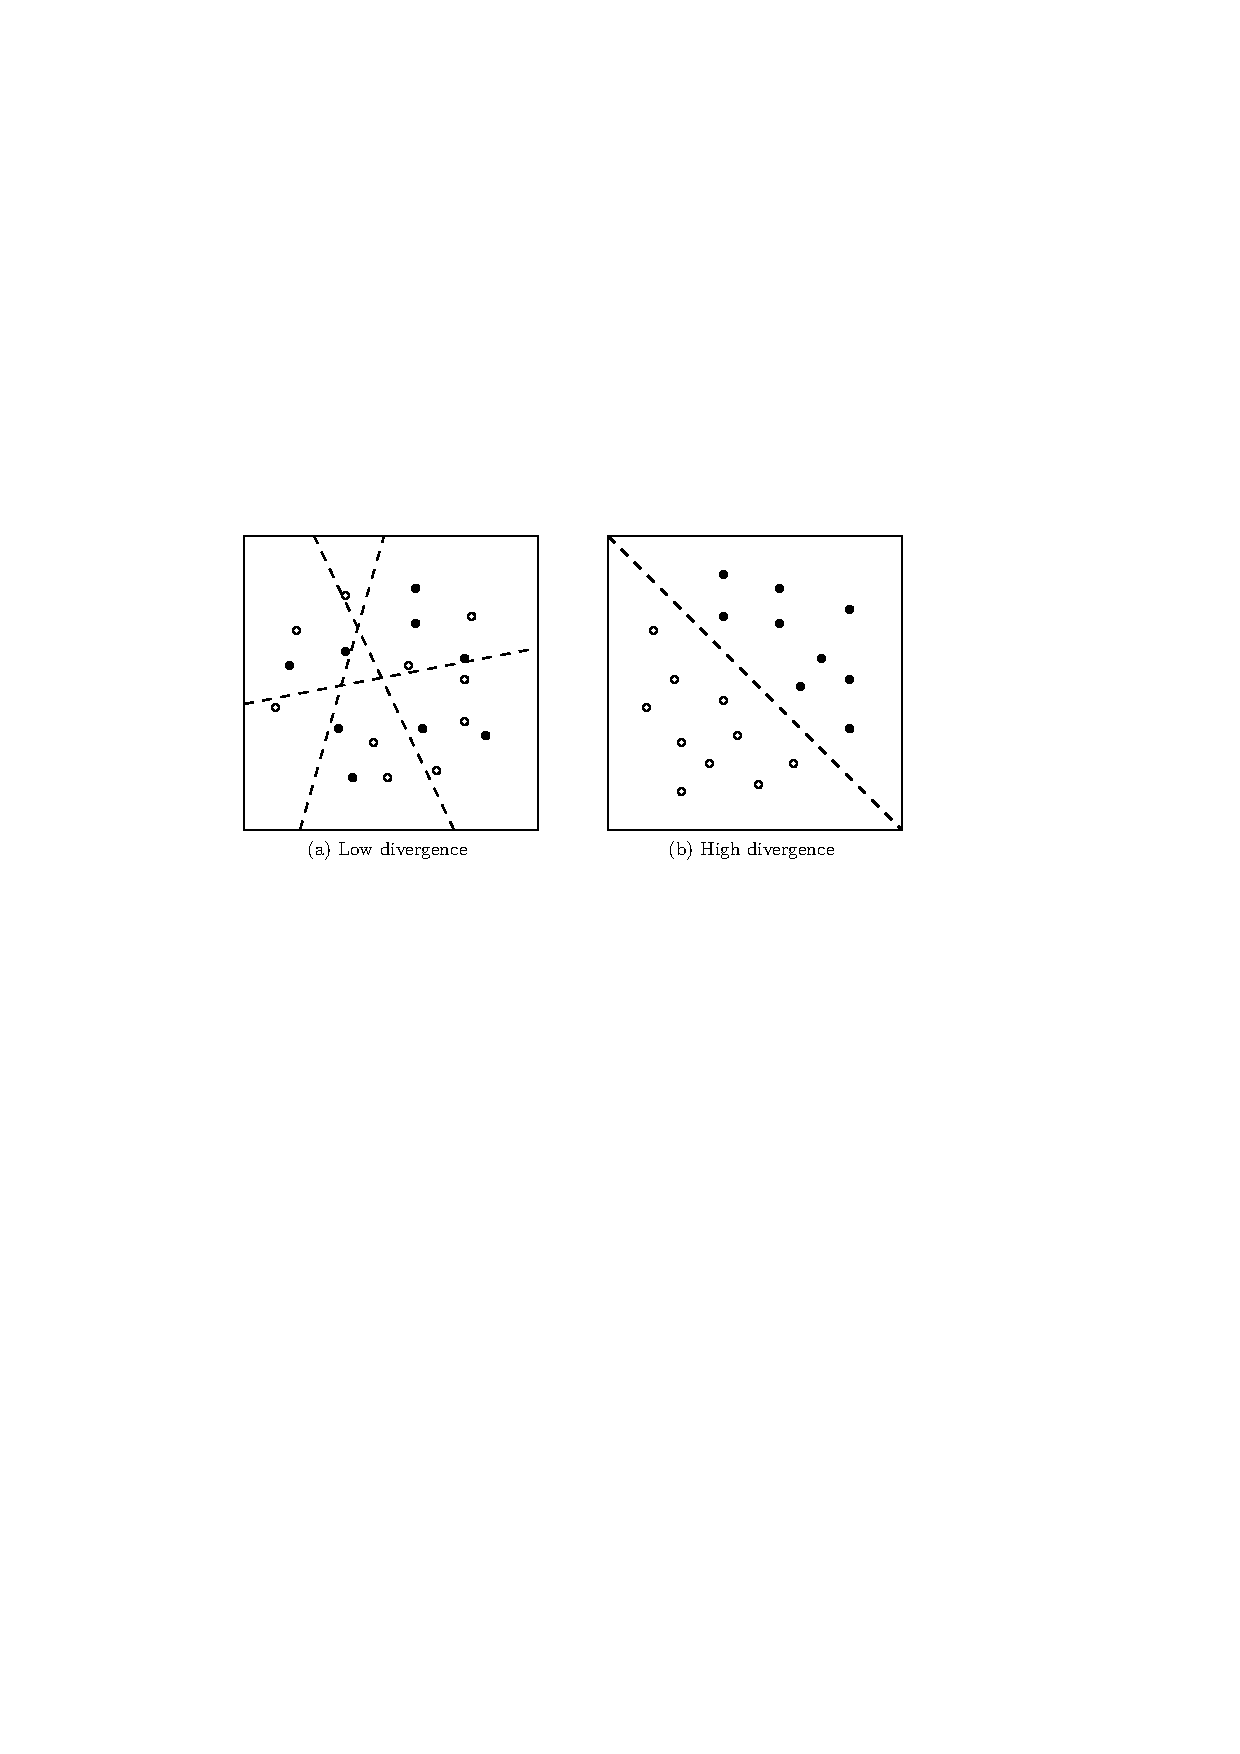
\includegraphics[width=0.7\textwidth]{../graphics/h_divergence.pdf}
   \caption{Illustration of h-divergence between domains.}
\end{figure}
\begin{itemize}
\item The divergence of domains can be quantified by trying to classify samples according to their source label. 
\item Hence, we train a classifier from a training set $T=\{(x_i, d_i)\}$: 
\begin{equation}
d_i= 
\begin{dcases}
    0,& \text{if } x_i \sim \mathcal{D}^X_S\\
    1,& \text{if } x_i \sim \mathcal{D}^X_T\\
\end{dcases}
\end{equation}
\item In this case, the h-divergence can be written as $2(1-2 \epsilon)$, where $\epsilon$ is the error of the classifier. 
\end{itemize}
\end{frame}

\begin{frame}{Domain adaptation by adversarial training}
\begin{figure}[htb]
   \centering
   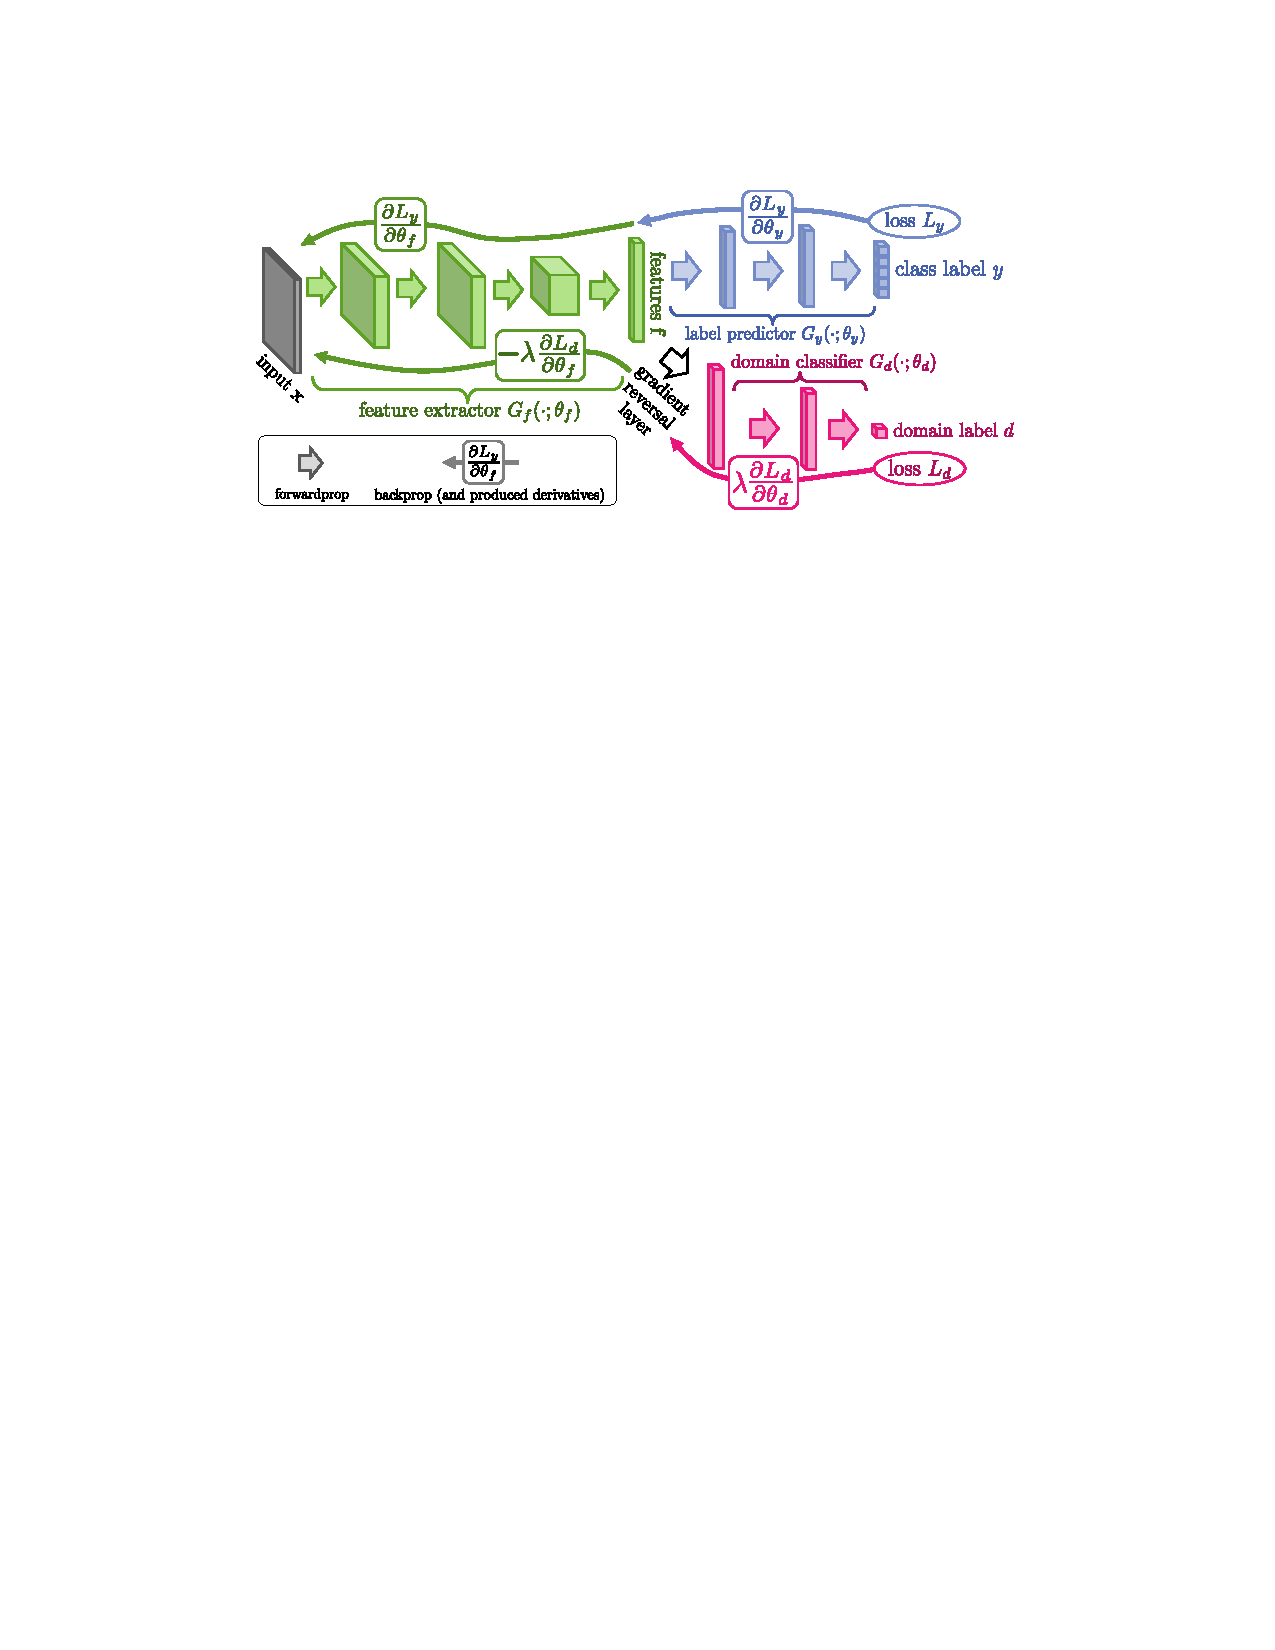
\includegraphics[width=0.7\textwidth]{../graphics/domain_adaptation.pdf}
   \caption{Domain adaptation by adversarial training. Image taken from \cite{Ganin2016}}
\end{figure}
\begin{itemize}
   \item We seek a representation that provides good prediction results, but low h-divergence. 
   \item This means that this representation ($f$ in the figure) should not allow us to distinguish between source domain and target domain. 
\end{itemize}
\end{frame}

\begin{frame}[noframenumbering]{Domain adaptation by adversarial training}
\begin{figure}[htb]
   \centering
   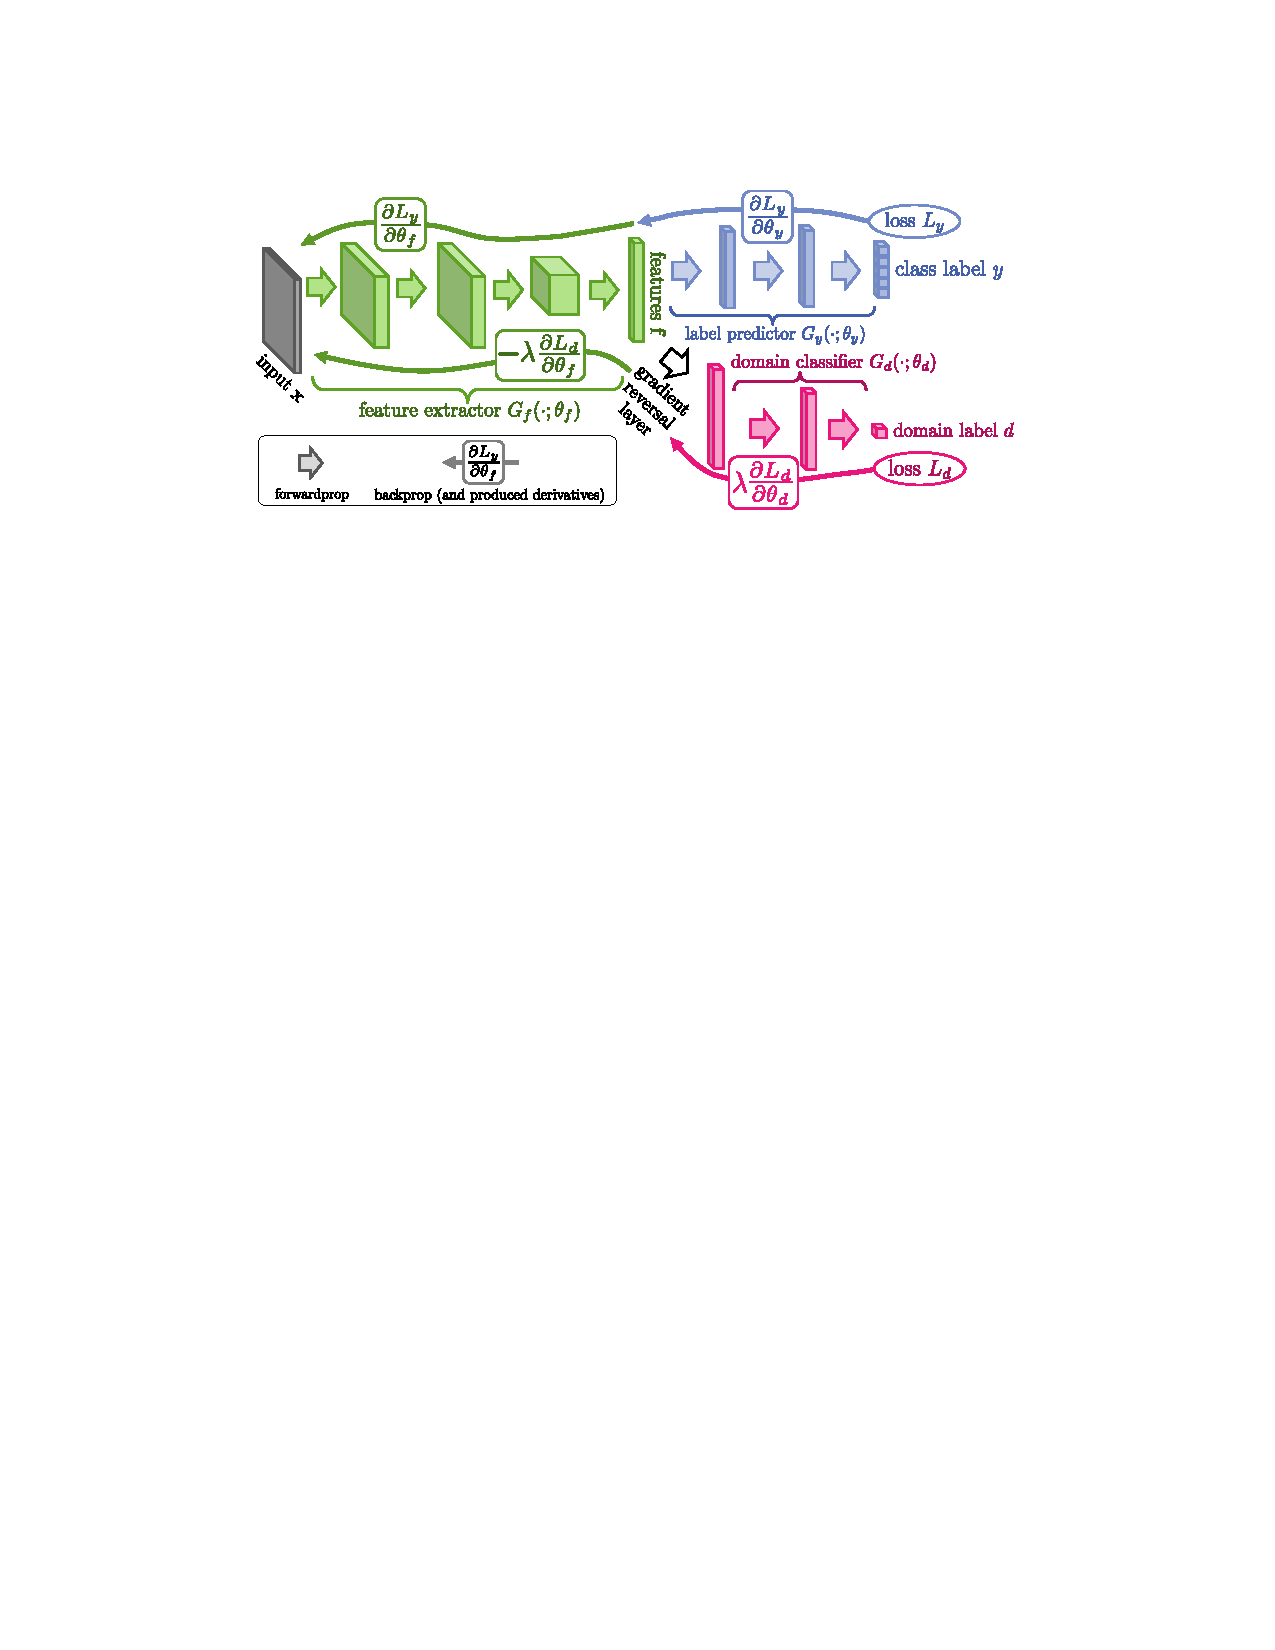
\includegraphics[width=0.7\textwidth]{../graphics/domain_adaptation.pdf}
   \caption{Domain adaptation by adversarial training. Image taken from \cite{Ganin2016}}
\end{figure}
For this we consider the following architecture \cite{Ganin2016}: 
\begin{itemize}
   \item $G_f(;,\theta_f)$ : feature extractor
   \item $G_y(;,\theta_y)$ : label predictor 
   \item $G_d(;,\theta_d)$ : domain classifier
\end{itemize}
\end{frame}

\begin{frame}[noframenumbering]{Domain adaptation by adversarial training}
\begin{figure}[htb]
   \centering
   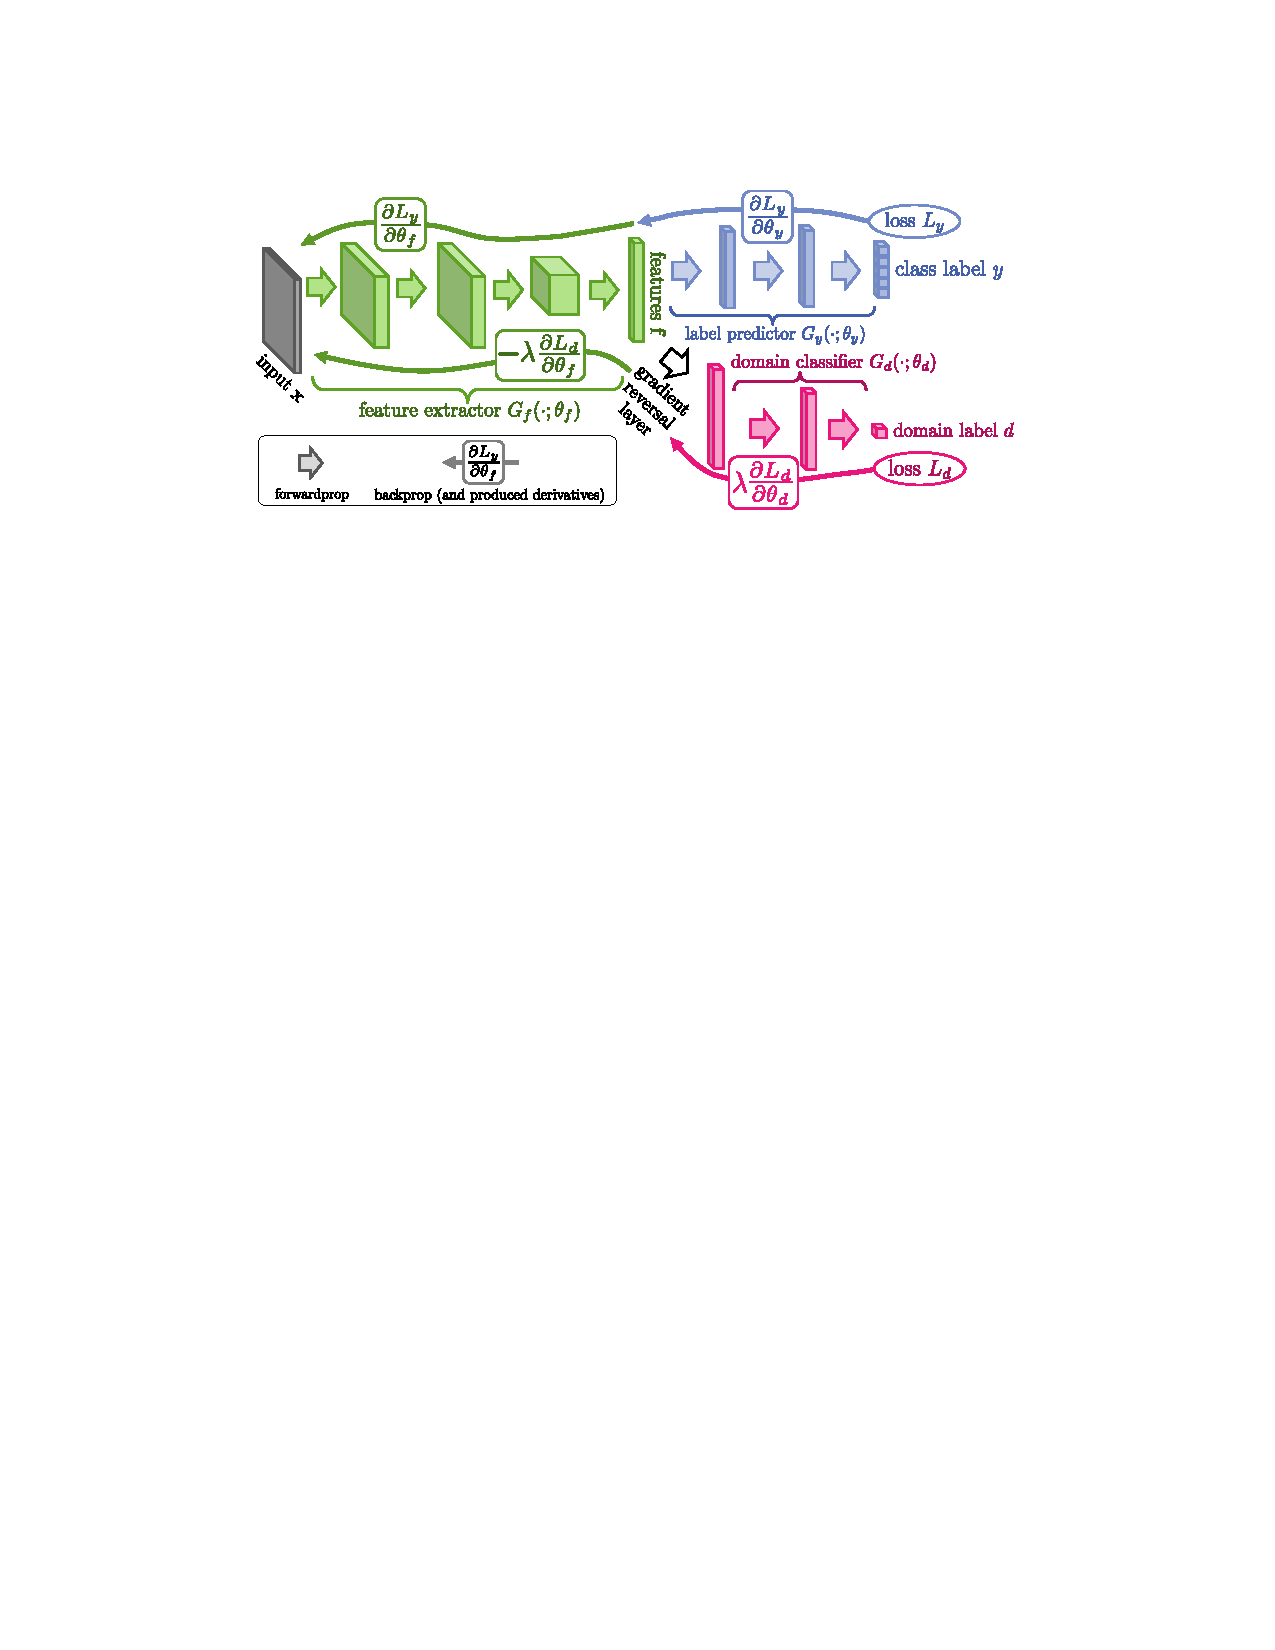
\includegraphics[width=0.7\textwidth]{../graphics/domain_adaptation.pdf}
   \caption{Domain adaptation by adversarial training. Image taken from \cite{Ganin2016}}
\end{figure}
The forward propagation produces then the following loss: 
\begin{equation}
\loss(\theta_f, \theta_y, \theta_d) = \loss_y(\theta_f, \theta_y) - \lambda \loss_d(\theta_f, \theta_d) 
\end{equation}
where $\loss_y(\theta_f, \theta_y)$ is the standard prediction loss for samples from the training set (and thus the source domain), while $\loss_d(\theta_f, \theta_d)$ is the domain loss, calculated on all samples (labeled samples from the source domain and the unlabeled samples from the target domain). 
\end{frame}

\begin{frame}{Domain adaptation by adversarial training - Optimization}
\begin{itemize}
   \item More formally, we write:
\begin{eqnarray*}
\loss_y(\theta_f, \theta_y) &=& \frac{1}{n} \sum_{i=1}^n \loss_y(G_y(G_f(x_i,\theta_f), \theta_y), y_i) \\
\loss_d(\theta_f, \theta_d) &=& \frac{1}{n} \sum_{i=1}^n \loss_d(G_d(G_f(x_i,\theta_f), \theta_d), d_i) \\
&+& \frac{1}{N-n} \sum_{i=n}^N\loss_d(G_d(G_f(x_i,\theta_f), \theta_d), d_i) \\
\loss(\theta_f, \theta_y, \theta_d) &=& \loss_y(\theta_f, \theta_y) - \lambda \loss_d(\theta_f, \theta_d) 
\end{eqnarray*}
\item This loss has to be minimized with respect to some parameters and maximized with respect to other parameters:
\begin{eqnarray*}
(\hat{\theta}_f, \hat{\theta}_y) &=& \argmin_{\theta_f, \theta_y} \loss(\theta_f, \theta_y, \hat{\theta}_d) \\
\hat{\theta}_d &=& \argmax_{\theta_d} \loss(\hat{\theta}_f, \hat{\theta}_y, \theta_d) \\
\end{eqnarray*}
\end{itemize}
\end{frame}

\begin{frame}{Domain adaptation by adversarial training - gradient reversal}
\begin{figure}[htb]
   \centering
   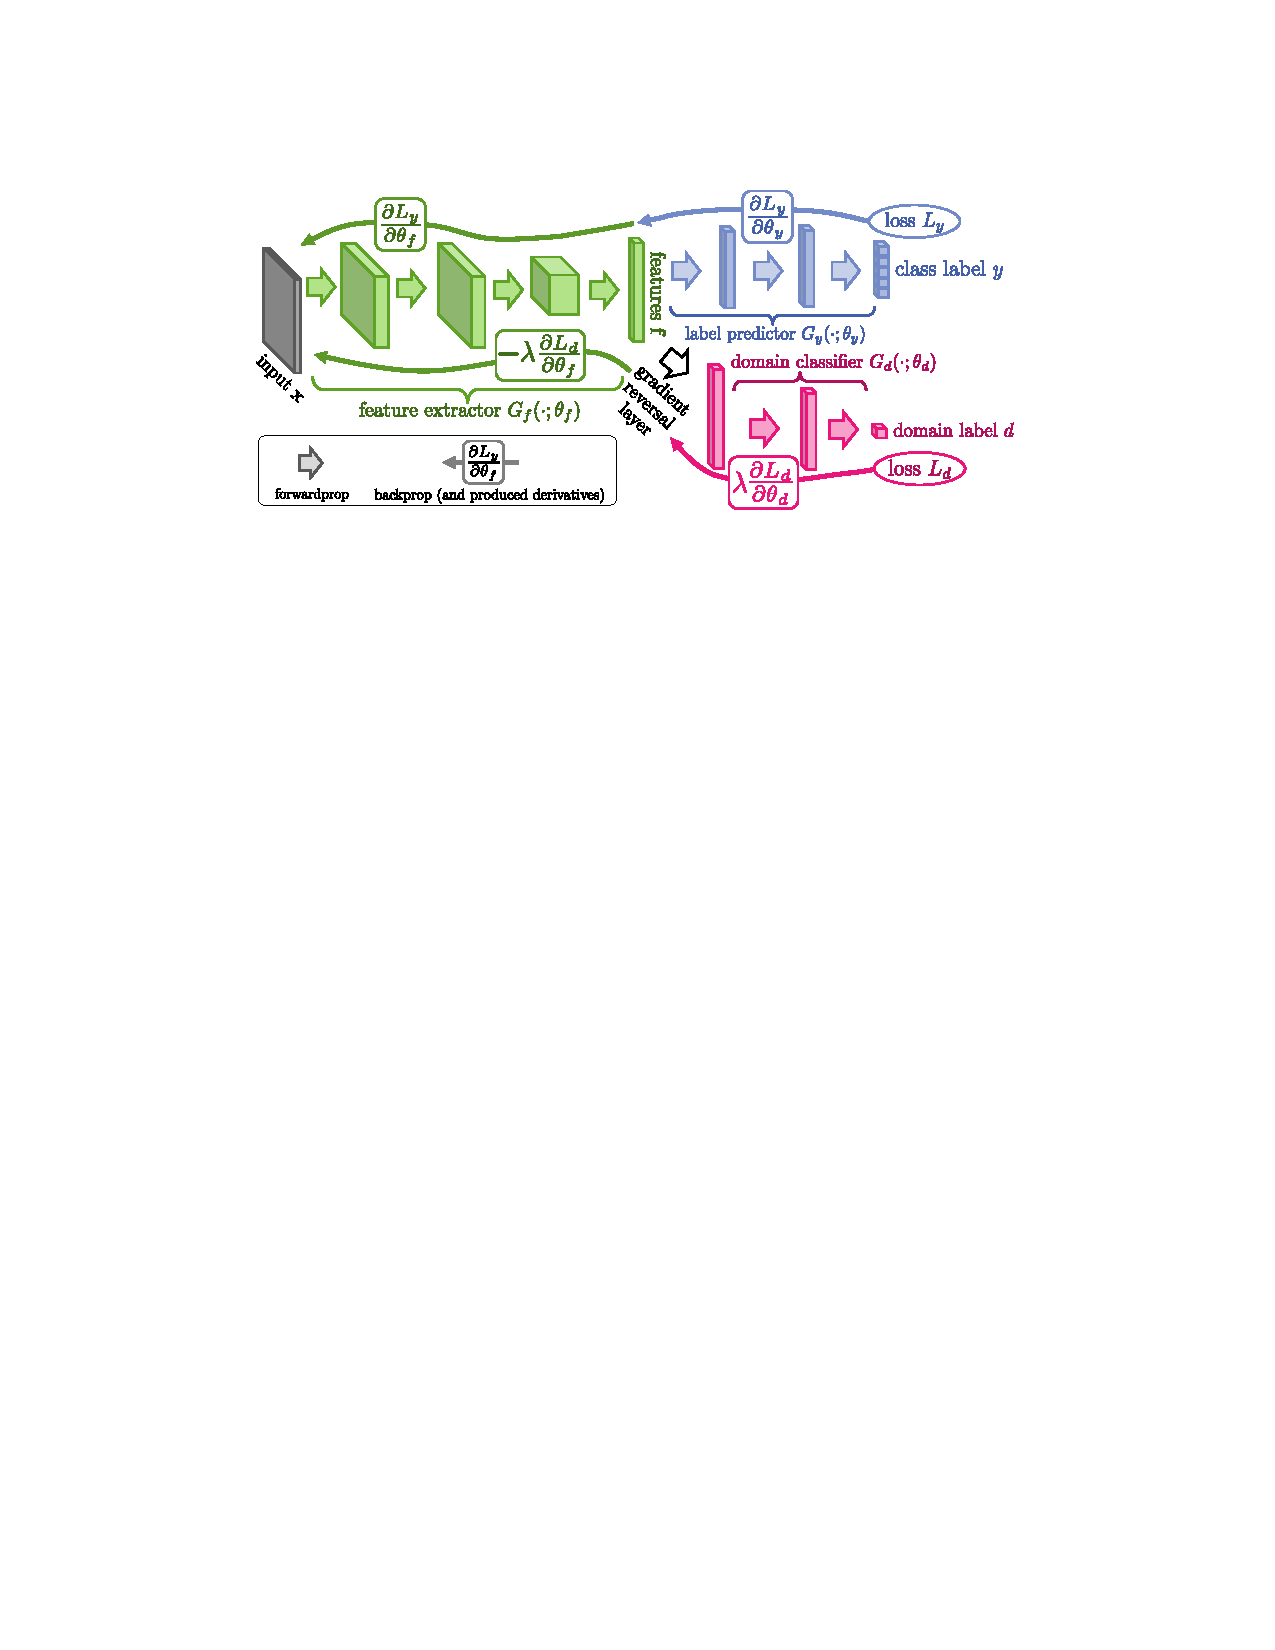
\includegraphics[width=0.7\textwidth]{../graphics/domain_adaptation.pdf}
   \caption{Domain adaptation by adversarial training. Image taken from \cite{Ganin2016}}
\end{figure}
The solution of simultaneous minimization and maximization can be elegantly solved by reversing a gradient layer during back-propagation, as indicated in the figure. 
\end{frame}

\begin{frame}{Application example: character classification}
\begin{figure}[htb]
   \centering
   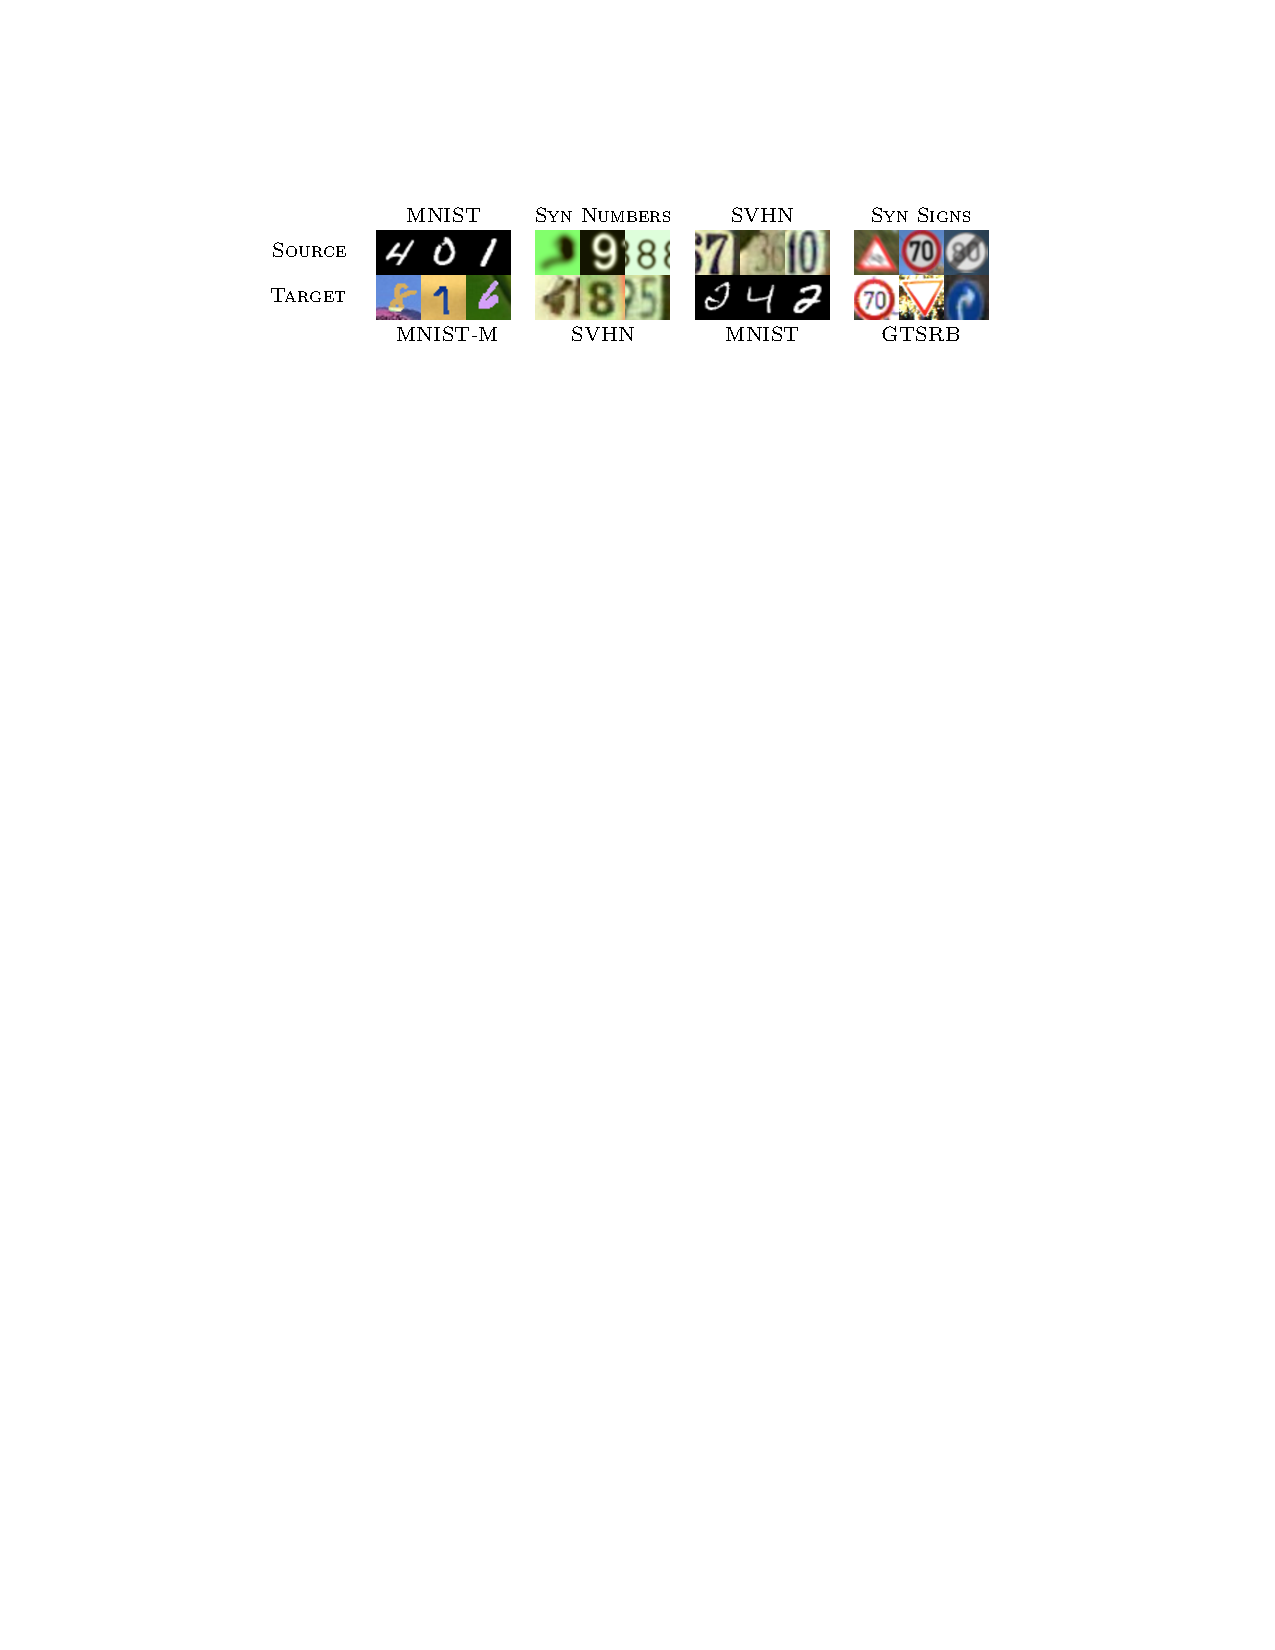
\includegraphics[width=0.7\textwidth]{../graphics/domain_adaptation_application.pdf}
   \caption{Domain adaptation between simulated and real data. MNIST: hand-written digits, MNIST-M: MNIST on top of random image patches, SYN Numbers: simulation created by varying Windows fonts, SVHN: street view house numbers, Image taken from \cite{Ganin2016}}
\end{figure}
Results indicate that the achievable improvements can reach up to $20\%$ in cases where the simulations are relatively far from the real-world examples. 
\end{frame}

\begin{frame}[noframenumbering]{Application example: character classification}
\begin{figure}[htb]
   \centering
   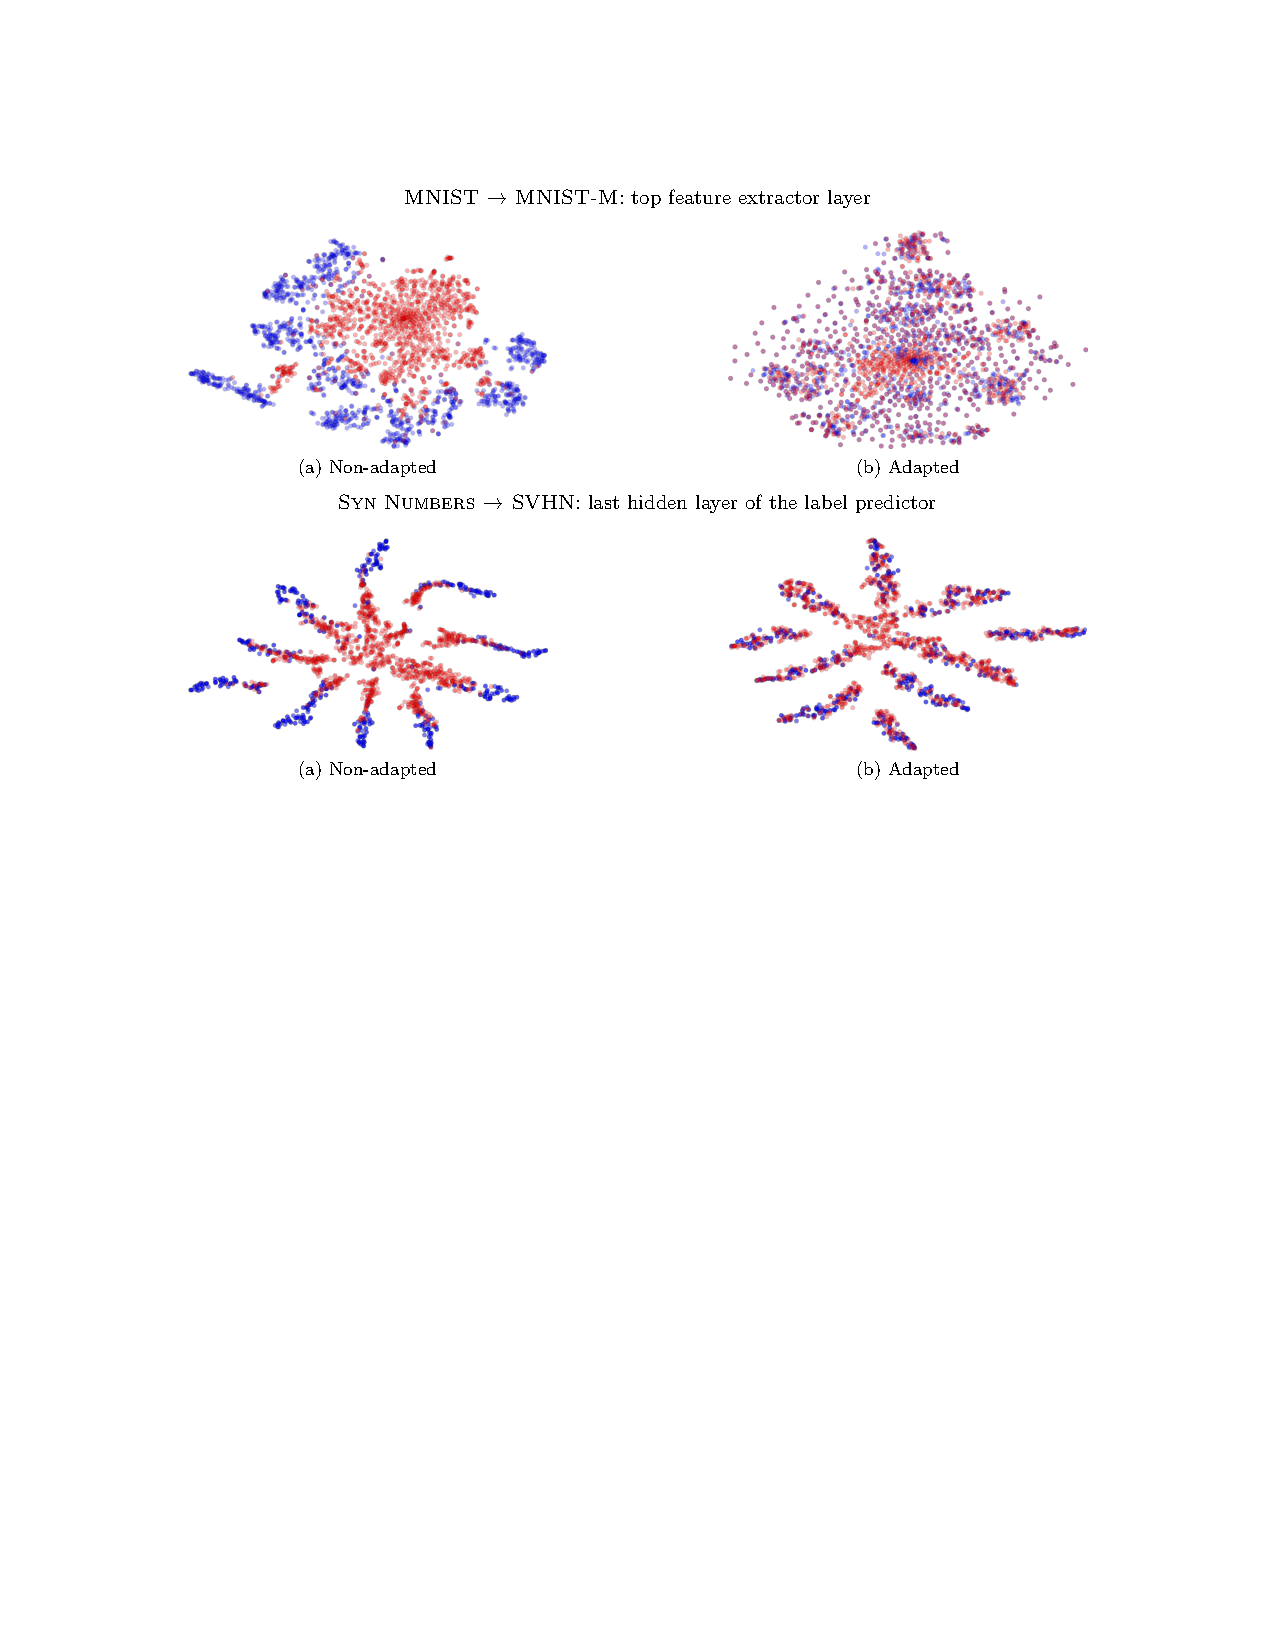
\includegraphics[width=0.9\textwidth]{../graphics/domain_adaptation_application_tsne.pdf}
   \caption{Learned representations with and without domain adaptation. Domains are colored in red and blue. Image taken from \cite{Ganin2016}.}
\end{figure}
\end{frame}

% \begin{frame}{Application example: character classification}
% \begin{figure}[htb]
%    \centering
%    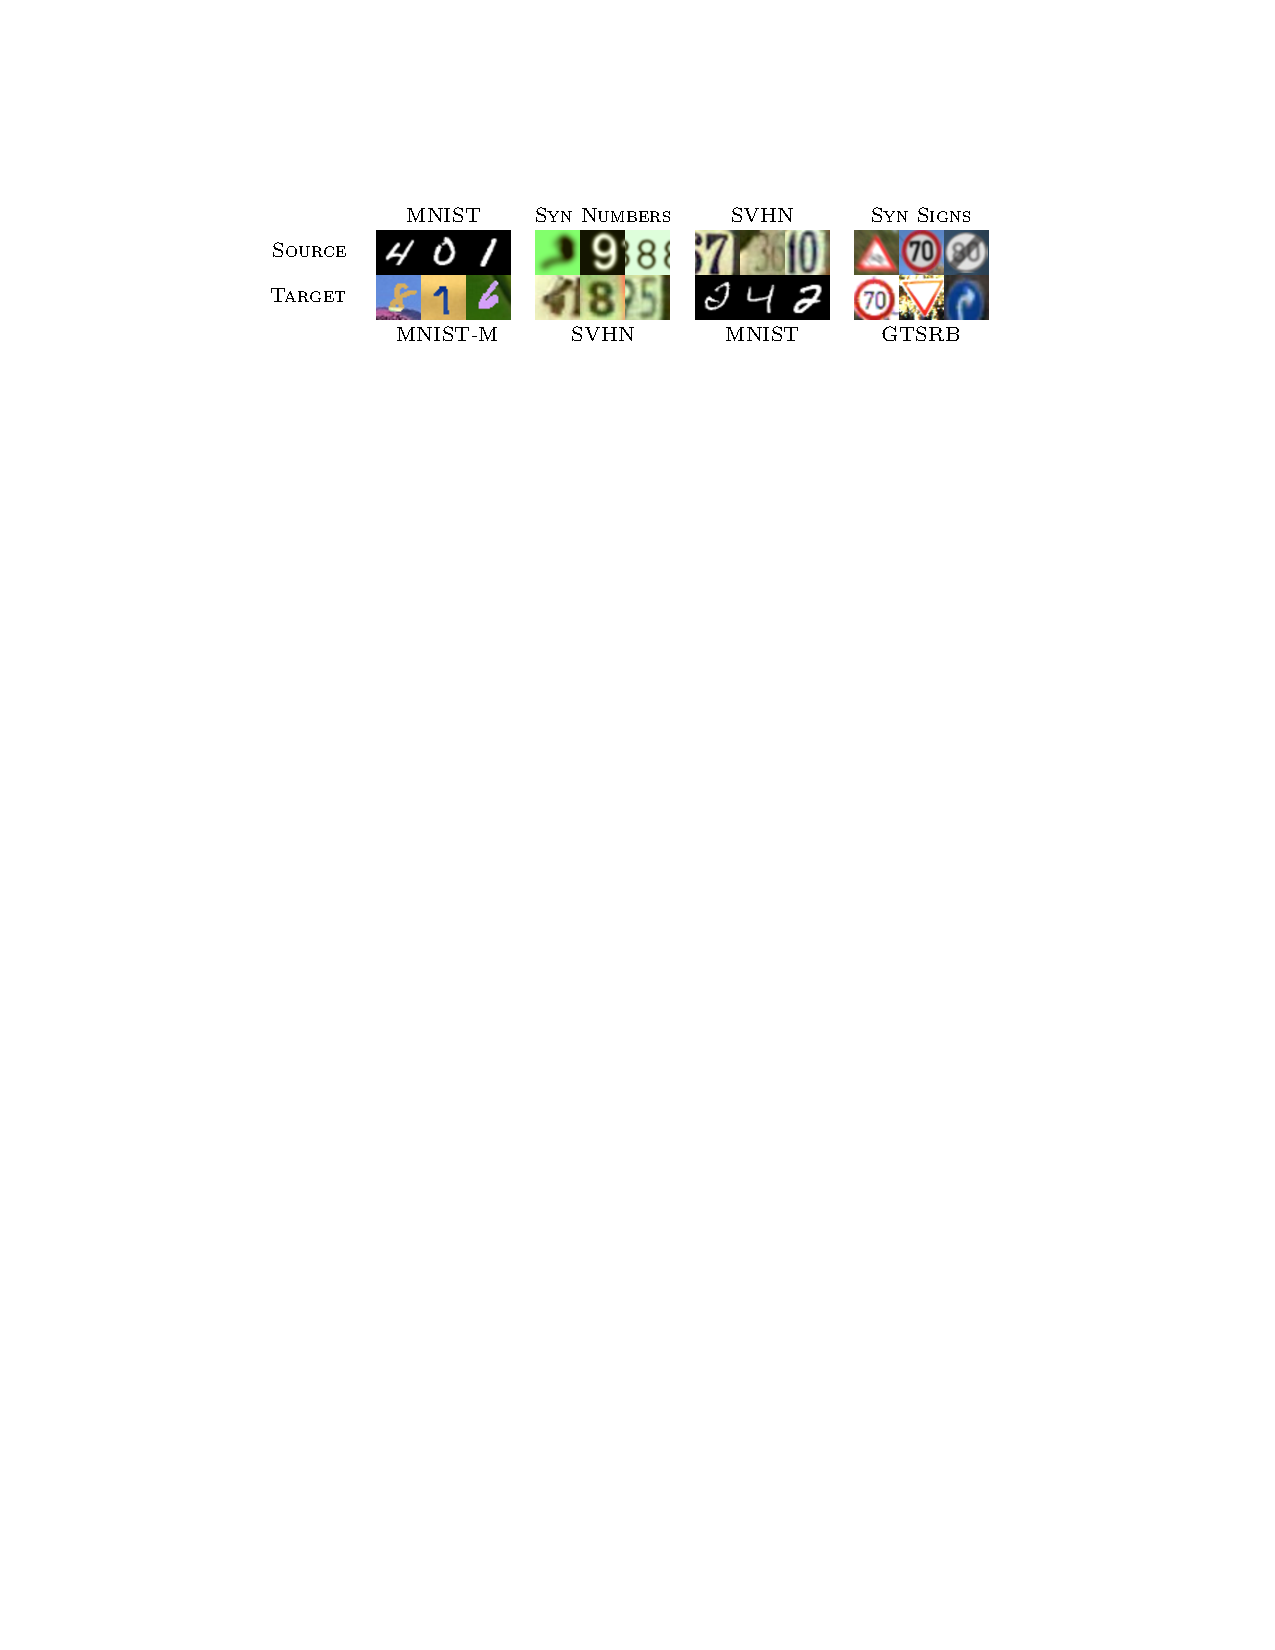
\includegraphics[width=0.7\textwidth]{../graphics/domain_adaptation_application.pdf}
%    \caption{Domain adaptation between simulated and real data. MNIST: hand-written digits, MNIST-M: MNIST on top of random image patches, SYN Numbers: simulation created by varying Windows fonts, SVHN: street view house numbers, Image taken from \cite{Ganin2016}}
% \end{figure}
% Results indicate that the achievable improvements can reach up to $20\%$ in cases where the simulations are relatively far from the real-world examples. 
% \end{frame}

% \begin{frame}{Application example: histopathology}

% \begin{itemize}
% \end{itemize}
% \end{frame}


%\cite{Oquab2015}

% \begin{frame}{Object detection: example}
% \begin{figure}[htb]
%    \centering
%    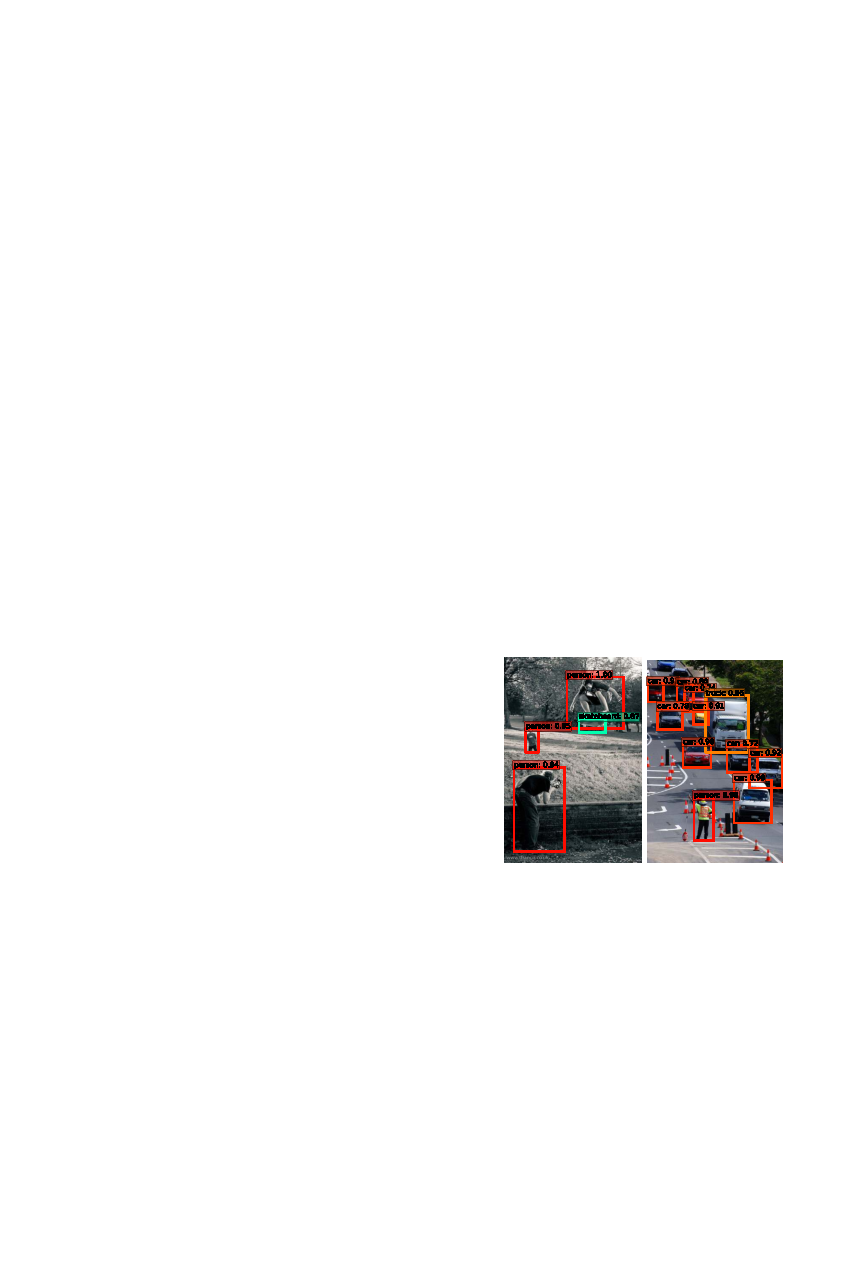
\includegraphics[width=0.95\textwidth]{../graphics/Detection_example1.pdf}
%    \caption{Object detection in action. Image taken from \cite{Liu2016}}
% \end{figure}
% \end{frame}


%The conv-layers are determined by first training the RPN (ImageNet initialization), then we train Fast R-CNN for the proposed regions (again with ImageNet initialization). The shared layers are then frozen.

%\item RPN and classification network thus share the conv-layers. They are specialized later. 

%%%%%%%%%%%%%%%%%%%%%%%%%%%%%%%%%%%%%%%%%%%%%%%%%%%%%%%%%%%%%%%%%%%%%%%%%
%%%%%%%%%%%%%%%%%%%%%%%%%%%%%%%%%%%%%%%%%%%%%%%%%%%%%%%%%%%%%%%%%%%%%%%%%
\section{Conclusion}
\frame{\frametitle{Overview}\tableofcontents[currentsection]}

\begin{frame}{Conclusion}
\begin{itemize}
   \item The need for large annotated data sets is currently a bottleneck in many real-world applications of deep learning. 
   \item There is a number of strategies to overcome massive manual image annotation. 
   \item Here, we have seen three strategies:
   \begin{enumerate}
      \item Contrastive Learning. 
      \item Learning from weakly supervised data
      \item Learning from simulations
   \end{enumerate}
   \item Usually, the way in which we setup the annotation strategy usually also influences the methodological developments. 
\end{itemize}
\end{frame}

%%%%%%%%%%%%%%%%%%%%%%%%%%%%%%%%%%%%%%%%%%%%%%%%%%%%%%%%%%%%%%%%%%%%%%%%%
%%%%%%%%%%%%%%%%%%%%%%%%%%%%%%%%%%%%%%%%%%%%%%%%%%%%%%%%%%%%%%%%%%%%%%%%%
\section{References}
\begin{frame}[allowframebreaks]
	\frametitle{References}
	\bibliography{weak_supervision_references.bib}
\end{frame}


\end{document}
